\documentclass[a4paper,12pt,oneside]{book} % nie: report!


% pakiety
\usepackage{polski} % lepiej to zamiast babel!
\usepackage[utf8]{inputenc} % w razie kłopotów spróbować: \usepackage[utf8x]{inputenc}
\usepackage{fancyhdr} % nagłówki i stopki
\usepackage{indentfirst} % WAŻNE, MA BYĆ!
\usepackage[pdftex]{graphicx} % to do wstawiania rysunków
\usepackage{amsmath} % to do dodatkowych symboli, przydatne
\usepackage[pdftex,
            left=1in,right=1in,
            top=1in,bottom=1in]{geometry} % marginsy
\usepackage{amssymb} % to też do dodatkowych symboli, też przydatne
\usepackage{pdfpages}
\usepackage{lipsum}
\usepackage{multirow}
\usepackage{listings}
\usepackage{caption}
\usepackage{booktabs}
\usepackage{subcaption}
\usepackage{xcolor}
\graphicspath{ {./pics/} }
\DeclareCaptionType{code}[Listing][Spis listingów] 

\definecolor{codegreen}{rgb}{0,0.6,0}
\definecolor{codegray}{rgb}{0.5,0.5,0.5}
\definecolor{codepurple}{rgb}{0.58,0,0.82}
\definecolor{backcolour}{rgb}{0.95,0.95,0.92}

% definicje nagłówków i stopek
\pagestyle{fancy}
\renewcommand{\chaptermark}[1]{\markboth{#1}{}}
\renewcommand{\sectionmark}[1]{\markright{\thesection\ #1}}
\fancyhf{}
\fancyhead[LE,RO]{\footnotesize\bfseries\thepage}
\fancyhead[LO]{\footnotesize\rightmark}
\fancyhead[RE]{\footnotesize\leftmark}
\renewcommand{\headrulewidth}{0.5pt}
\renewcommand{\footrulewidth}{0pt}
\addtolength{\headheight}{1.5pt}
\fancypagestyle{plain}{\fancyhead{}\cfoot{\footnotesize\bfseries\thepage}\renewcommand{\headrulewidth}{0pt}}


% interlinia
\linespread{1.25}

\title{Aplikacja dla stworzenia planu zajęć. Dokumentacja}
\author{Aleh Hutsko}

% treść
\begin{document}


\maketitle

\tableofcontents{}

\chapter*{Pierwsze zagadnenia}
Aplikacja dla stworzenia planu zajęć. Rejestracja/Logowanie, zapisywanie planu na konto, kilka typów planów (np. na różne tygodnie, semestry, itd.)

\addcontentsline{toc}{chapter}{Pierwsze zagadnenia}

\chapter*{Opis aplikacji}

Utworzono aplikację z możliwością logowania i rejestracji oraz z możliwością tworzenia kilku prywatnych (widocznych tylko dla twórcy planu) planów.
Plany są zapisywane w bazie danych. Dodano także możliwość dodawania przedmiotów do konta.
Utworzone przedmioty są wykorzystywane do tworzenia planu.

Wykorzystane technologii/narzędzia:
\begin{itemize}
    \item Visual Studio 2022
    \item Microsoft SQL Server Management Studio 18
    \item .NET Core MVC 
    \item C\# 10 (.NET 6.0)
    \item Entity Framework Core
    \item SQL Server
    \item Bootstrap
\end{itemize}

Aplikacja ....:

\begin{itemize}
    \item wykorzysta SQL server, (więc dla działania musimy mieć SQL Server na urządzeniu, na którym chcemy właczyć aplikacje)
    \item jest typu MVC,
    \item spełnia warunki CRUD
    \item ma 4 modele danych (4 tabeli w BD) (Rysunek \ref{fig:modele}),
    \item ma funkcje logowania/rejestracji.
\end{itemize}

\begin{figure}[h]
    \centering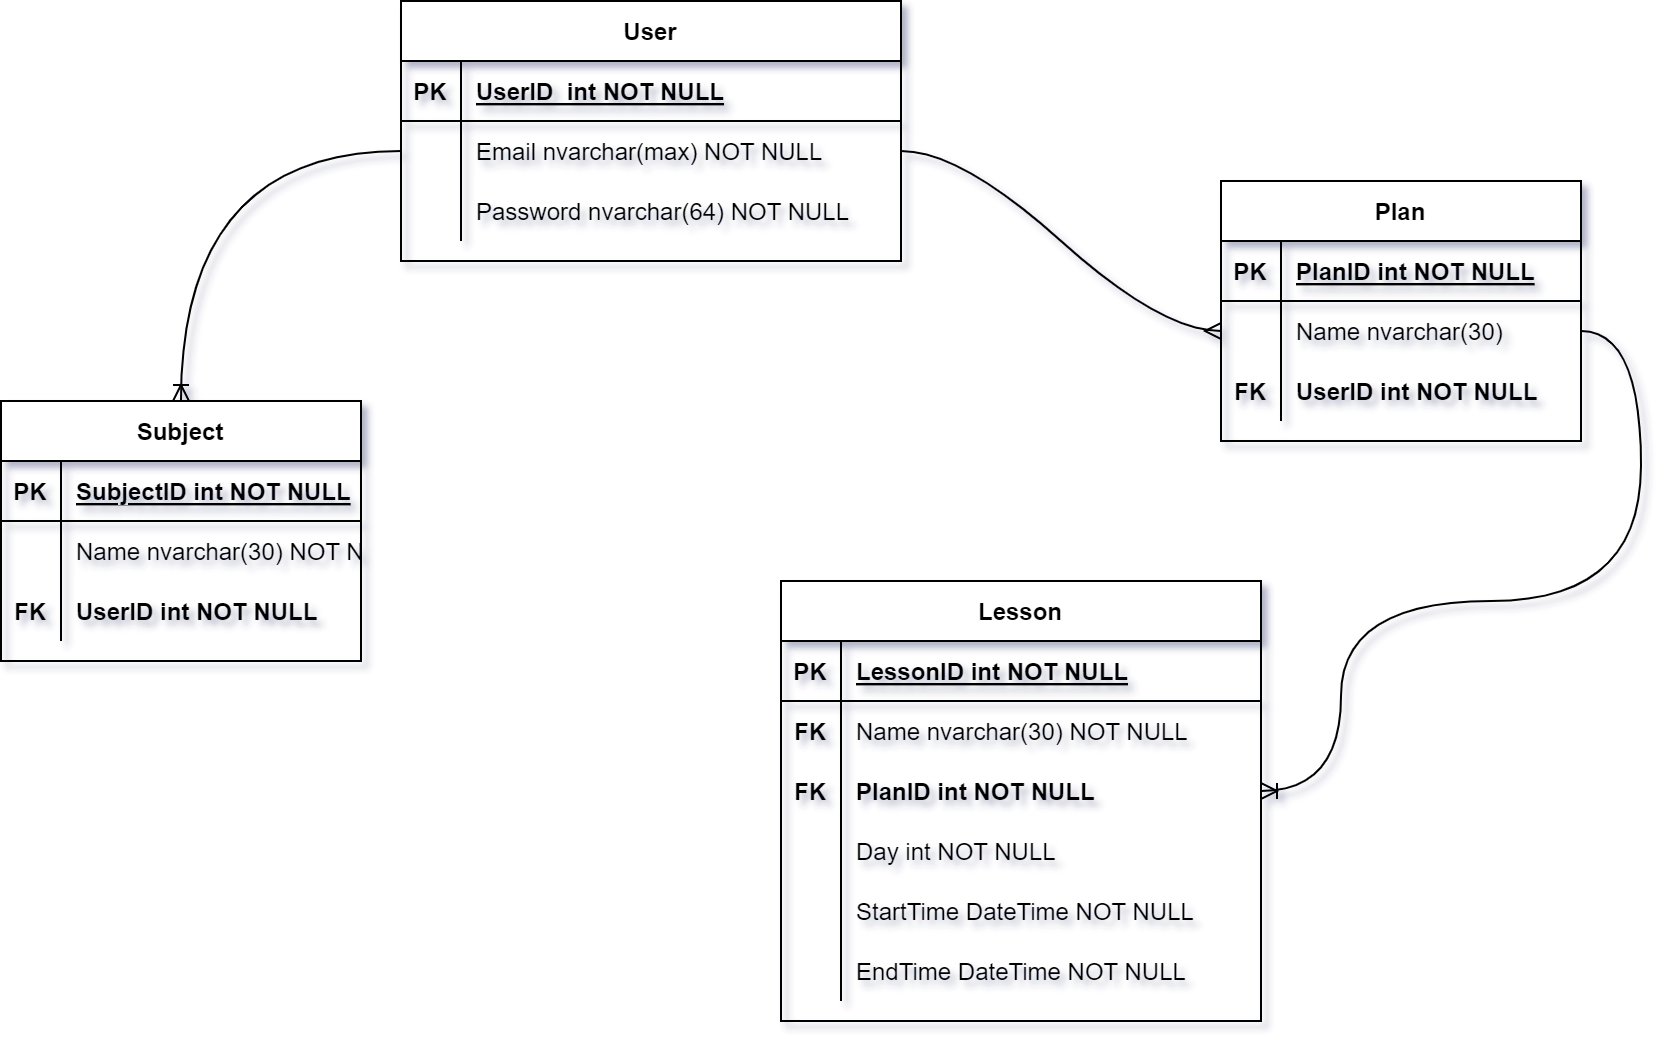
\includegraphics[width=14cm]{entities.png}
    \caption{Modeli danych}
    \label{fig:modele}
\end{figure}

\addcontentsline{toc}{chapter}{Krótki opis aplikacji}
\chapter*{Rejestracja/Logowanie}


\begin{figure}[h]
    \centering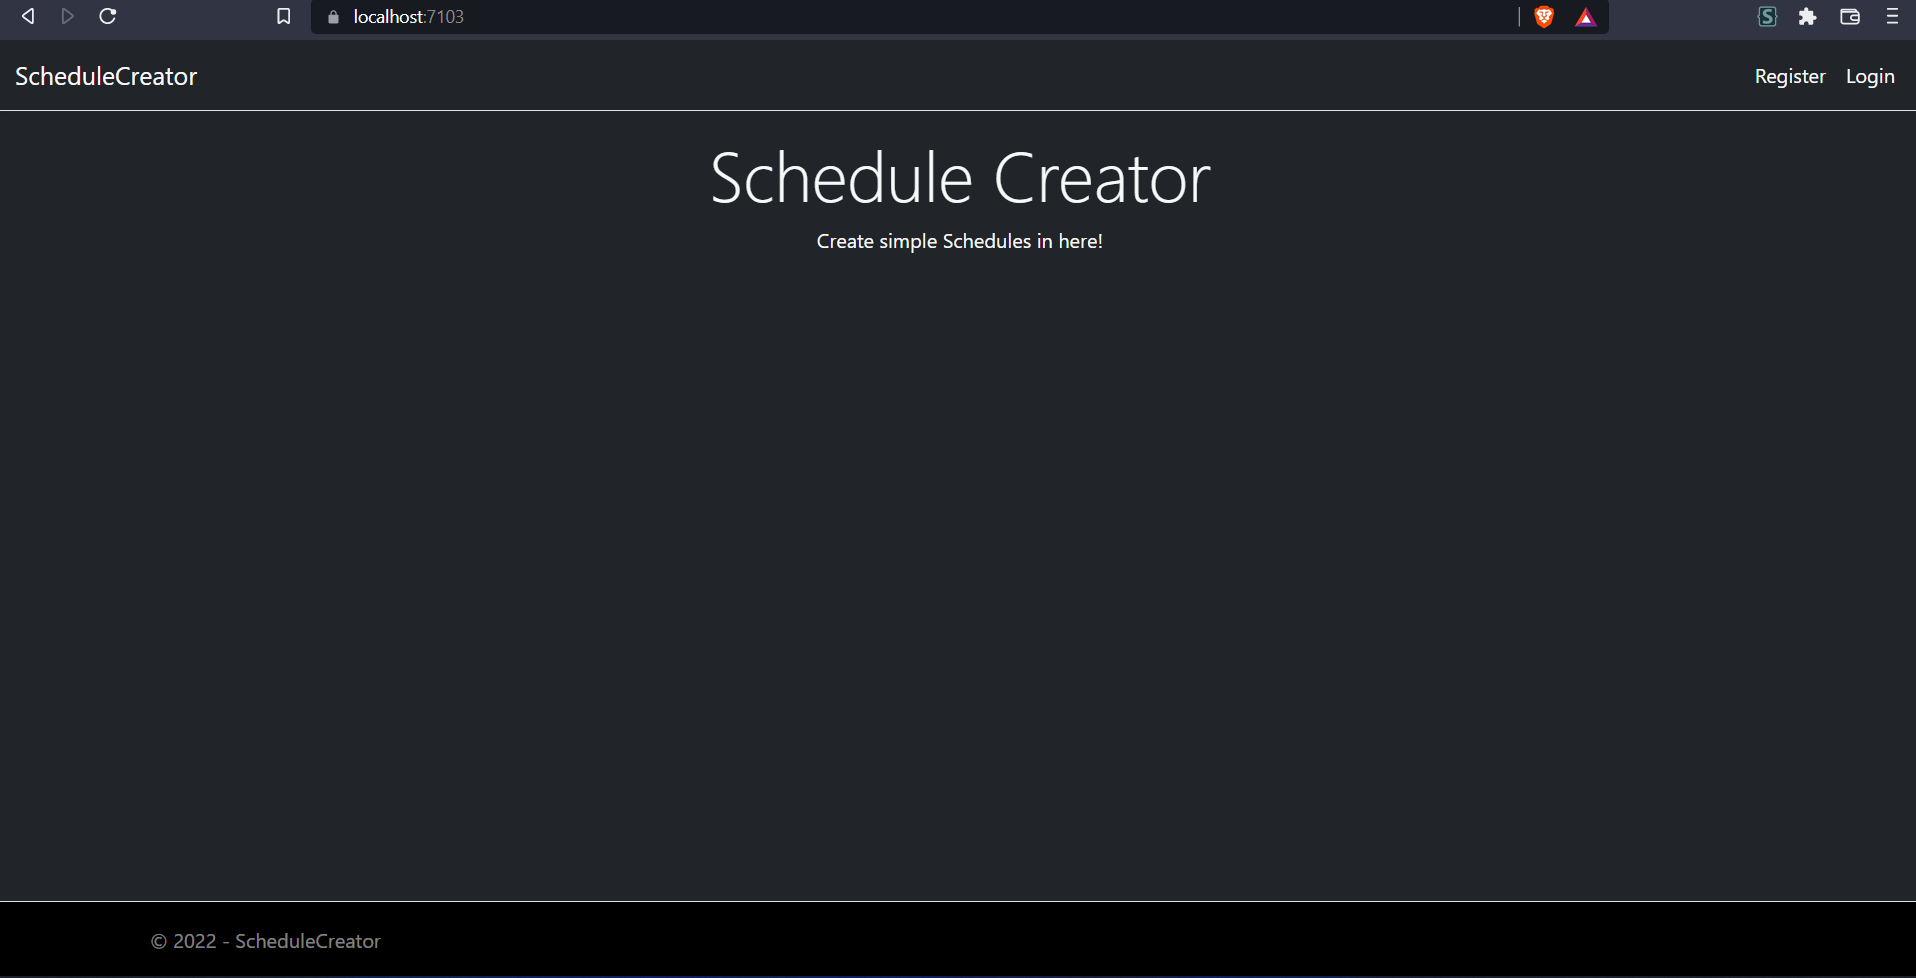
\includegraphics[width=14cm]{1.png}
    \caption{Strona główna}
\end{figure}

\begin{figure}[h]
    \centering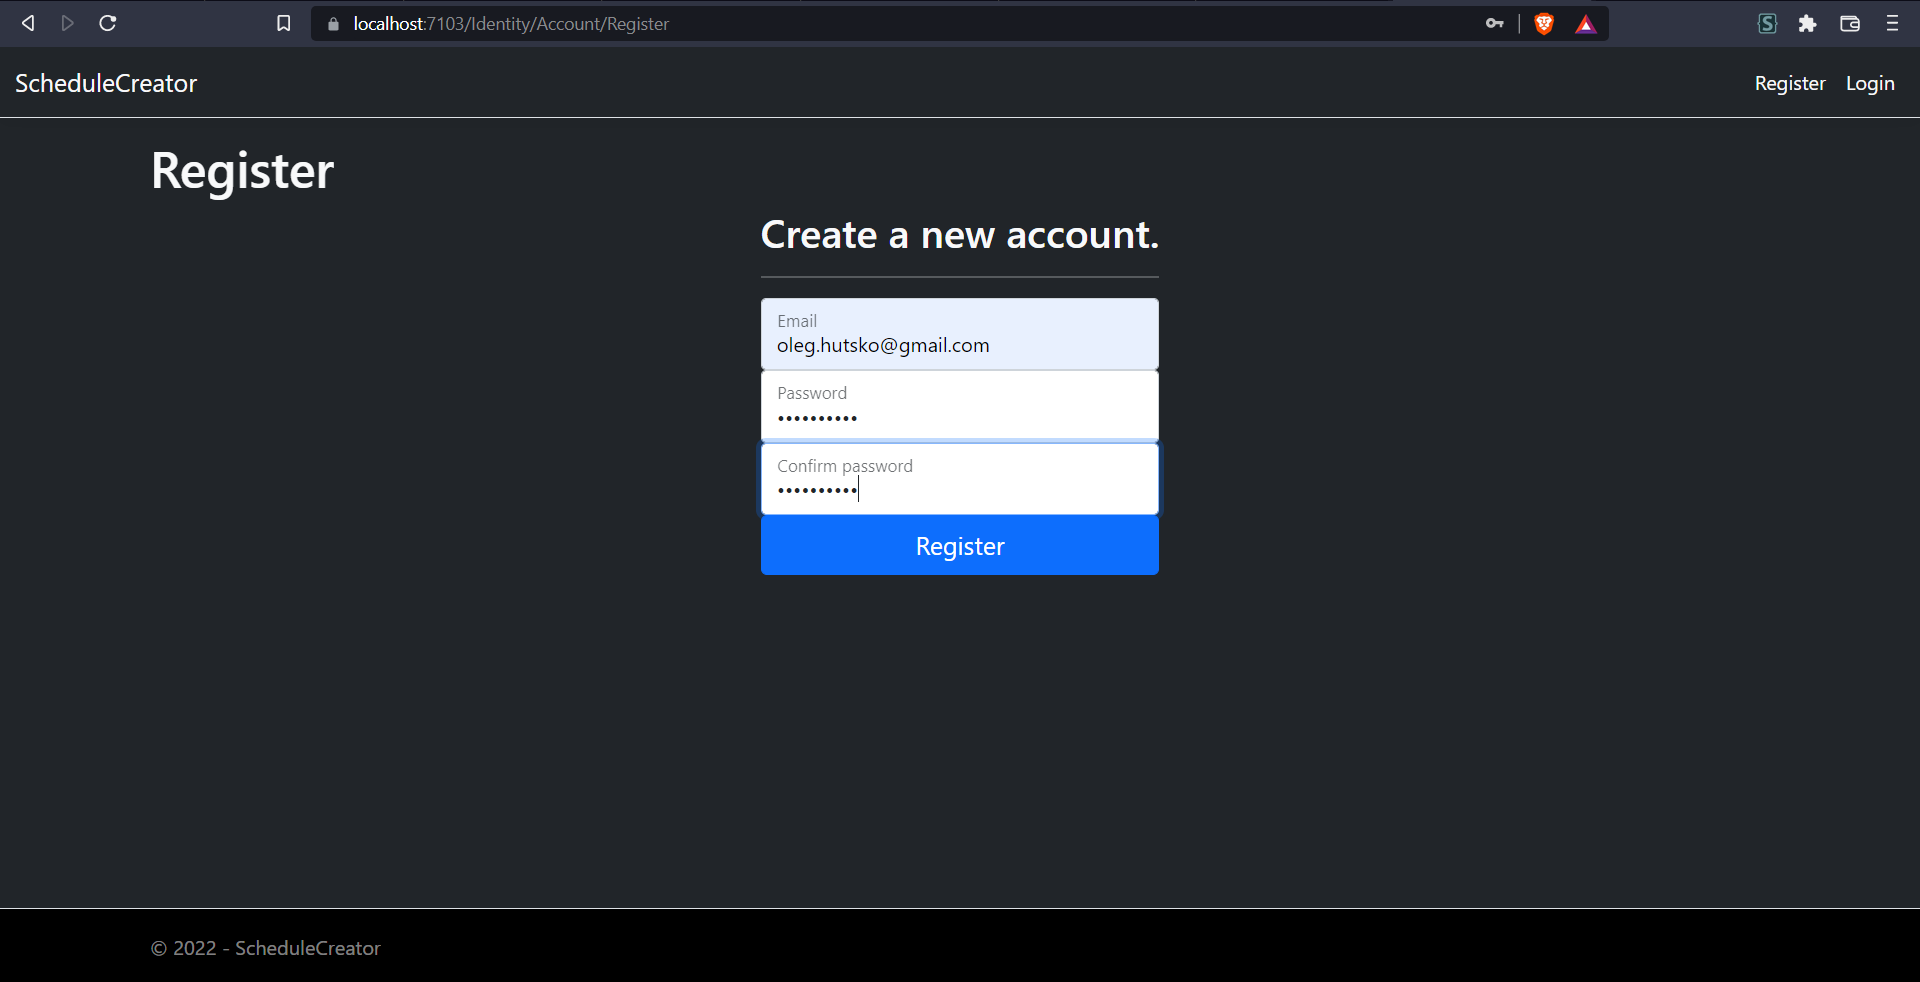
\includegraphics[width=14cm]{2.png}
    \caption{Strona rejestracji}
\end{figure}


\begin{figure}[h]
    \centering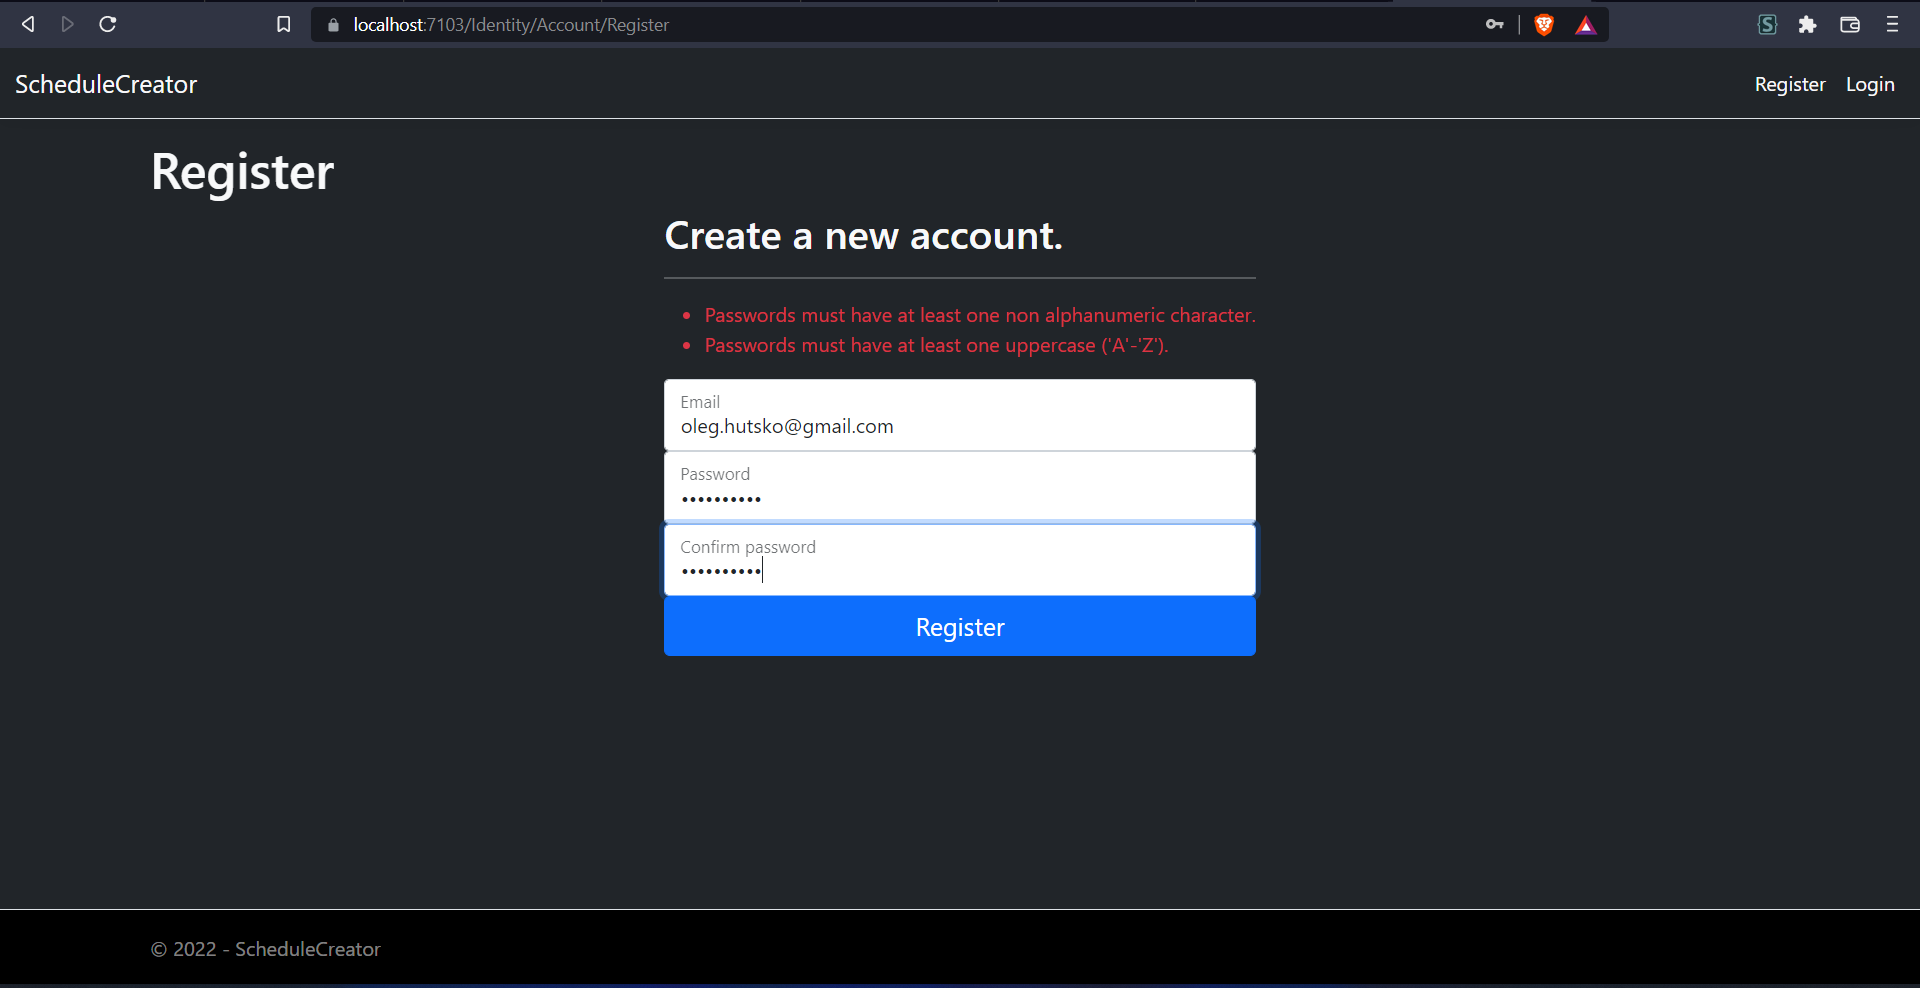
\includegraphics[width=14cm]{3.png}
    \caption{Nieudana rejestracja}
\end{figure}

\begin{figure}[h]
    \centering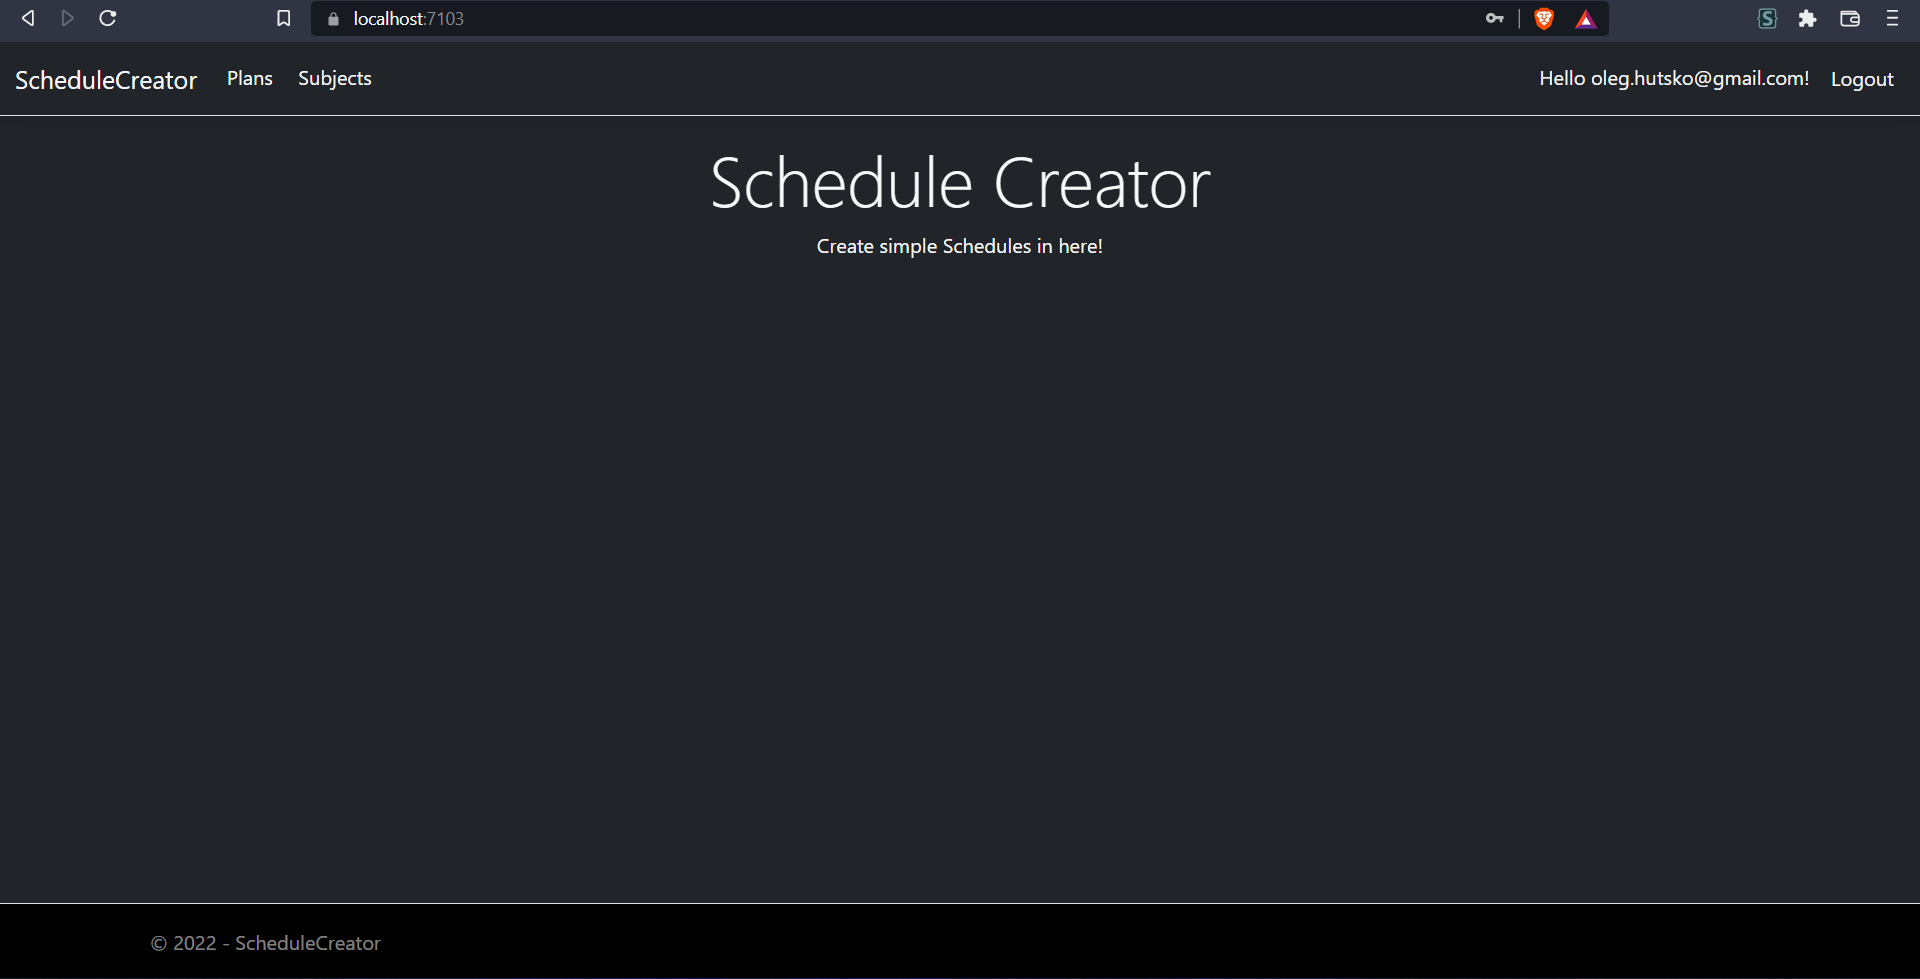
\includegraphics[width=14cm]{4.png}
    \caption{Po udanej rejestacji następuje automatyczne logowanie, głowna strona po zalogowaniu}
\end{figure}

\begin{figure}[h]
    \centering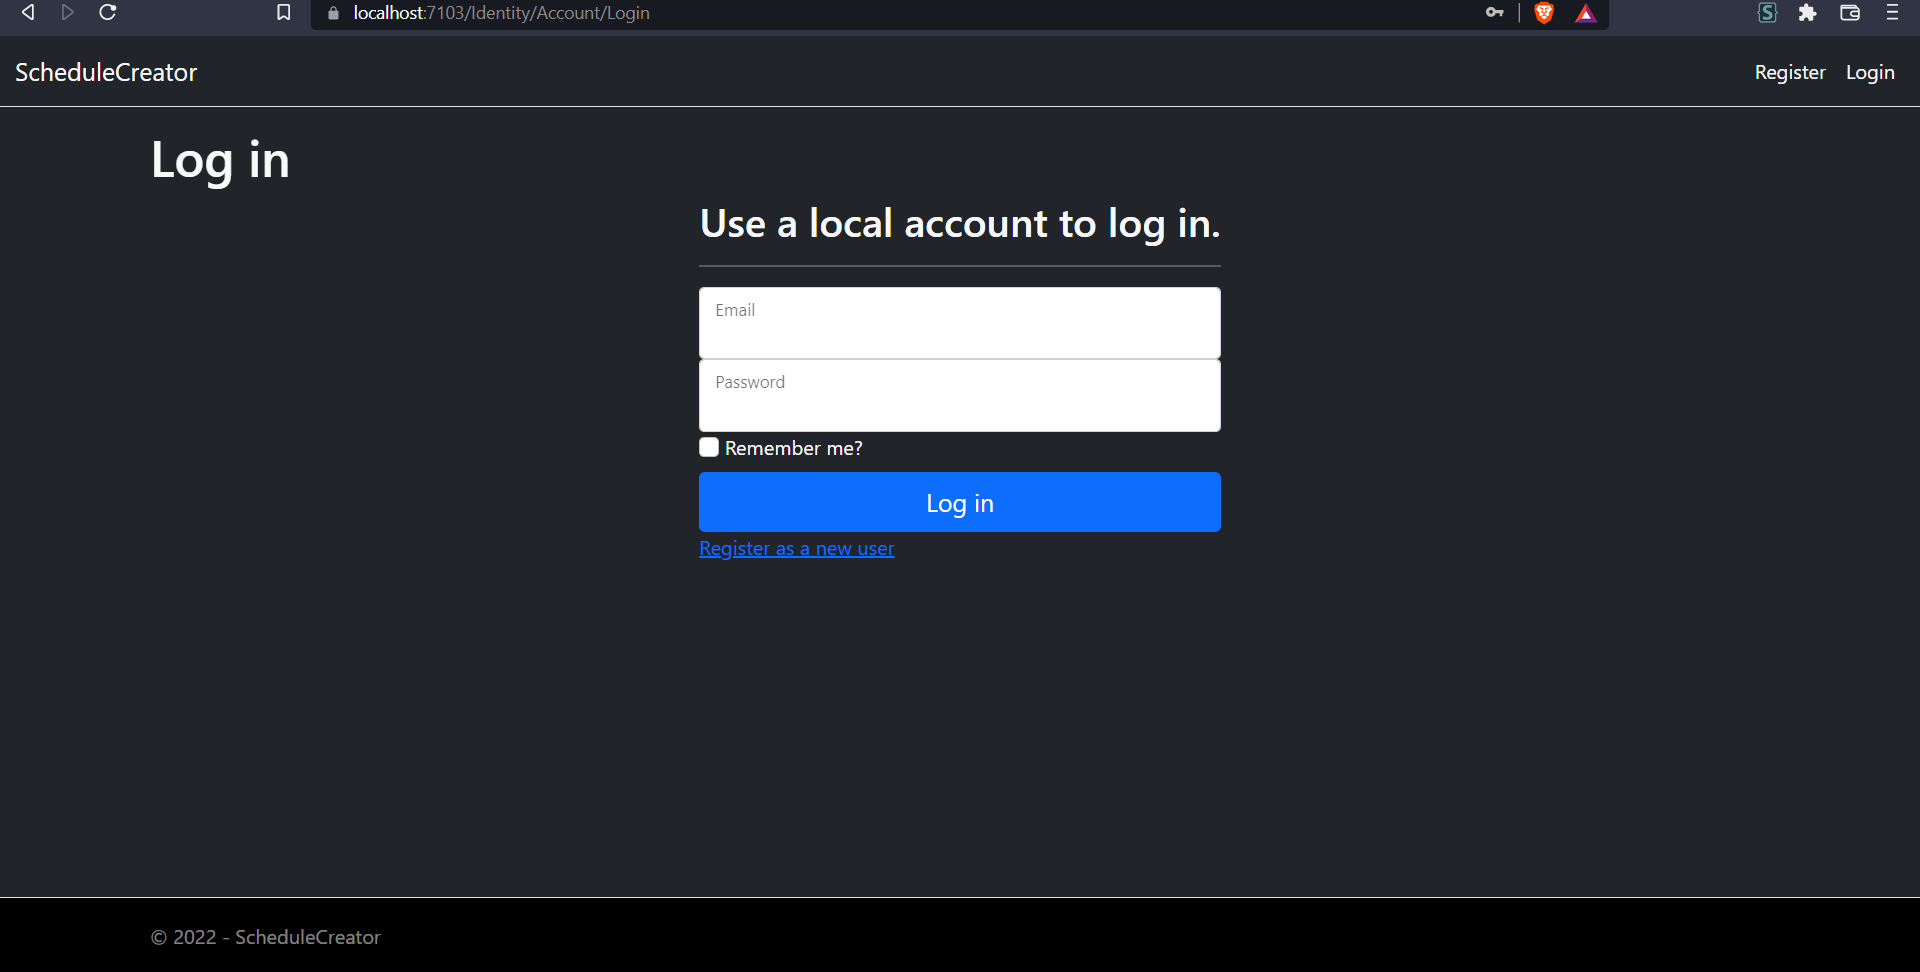
\includegraphics[width=14cm]{5.png}
    \caption{Strona logowania}
\end{figure}

\addcontentsline{toc}{chapter}{Rejestracja/Logowanie}
\chapter*{CRUD przedmioty}

\begin{figure}[h]
    \centering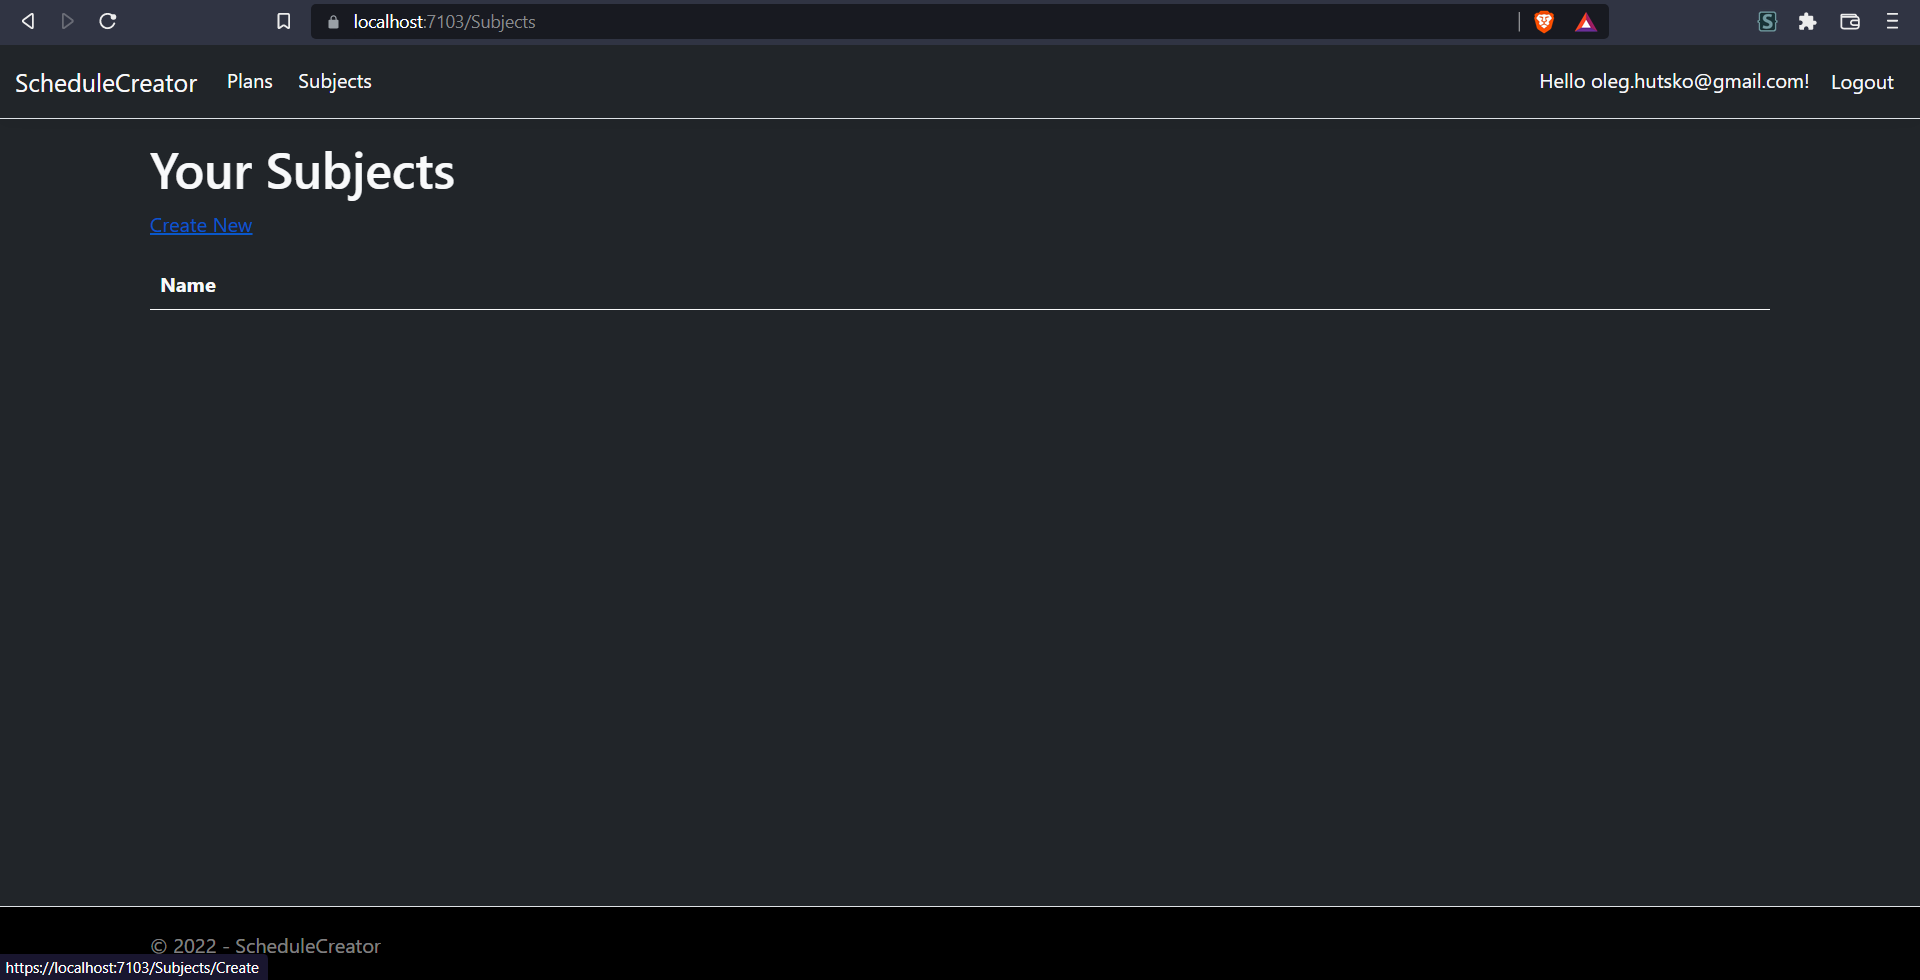
\includegraphics[width=14cm]{6.png}
    \caption{Strona przedmiotów (pusta)}
\end{figure}

\begin{figure}[h]
    \centering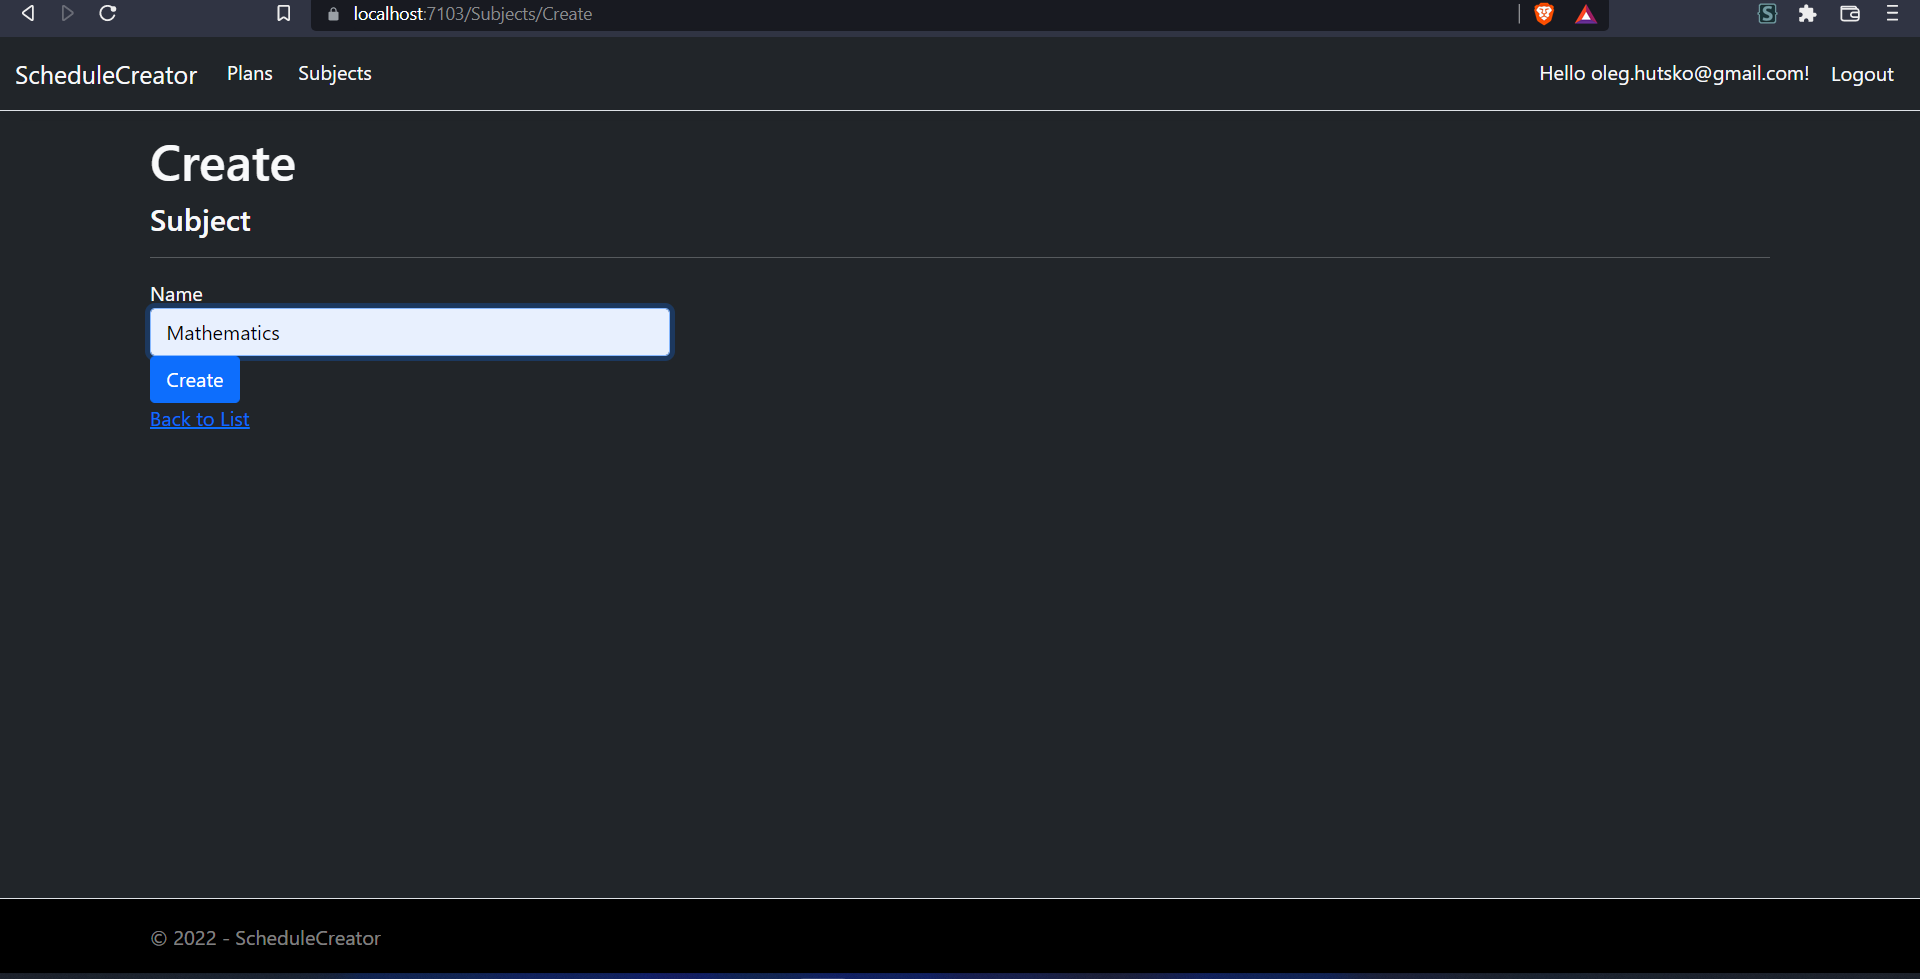
\includegraphics[width=14cm]{7.png}
    \caption{Strona stworzenia przedmiotów}
\end{figure}


\begin{figure}[h]
    \centering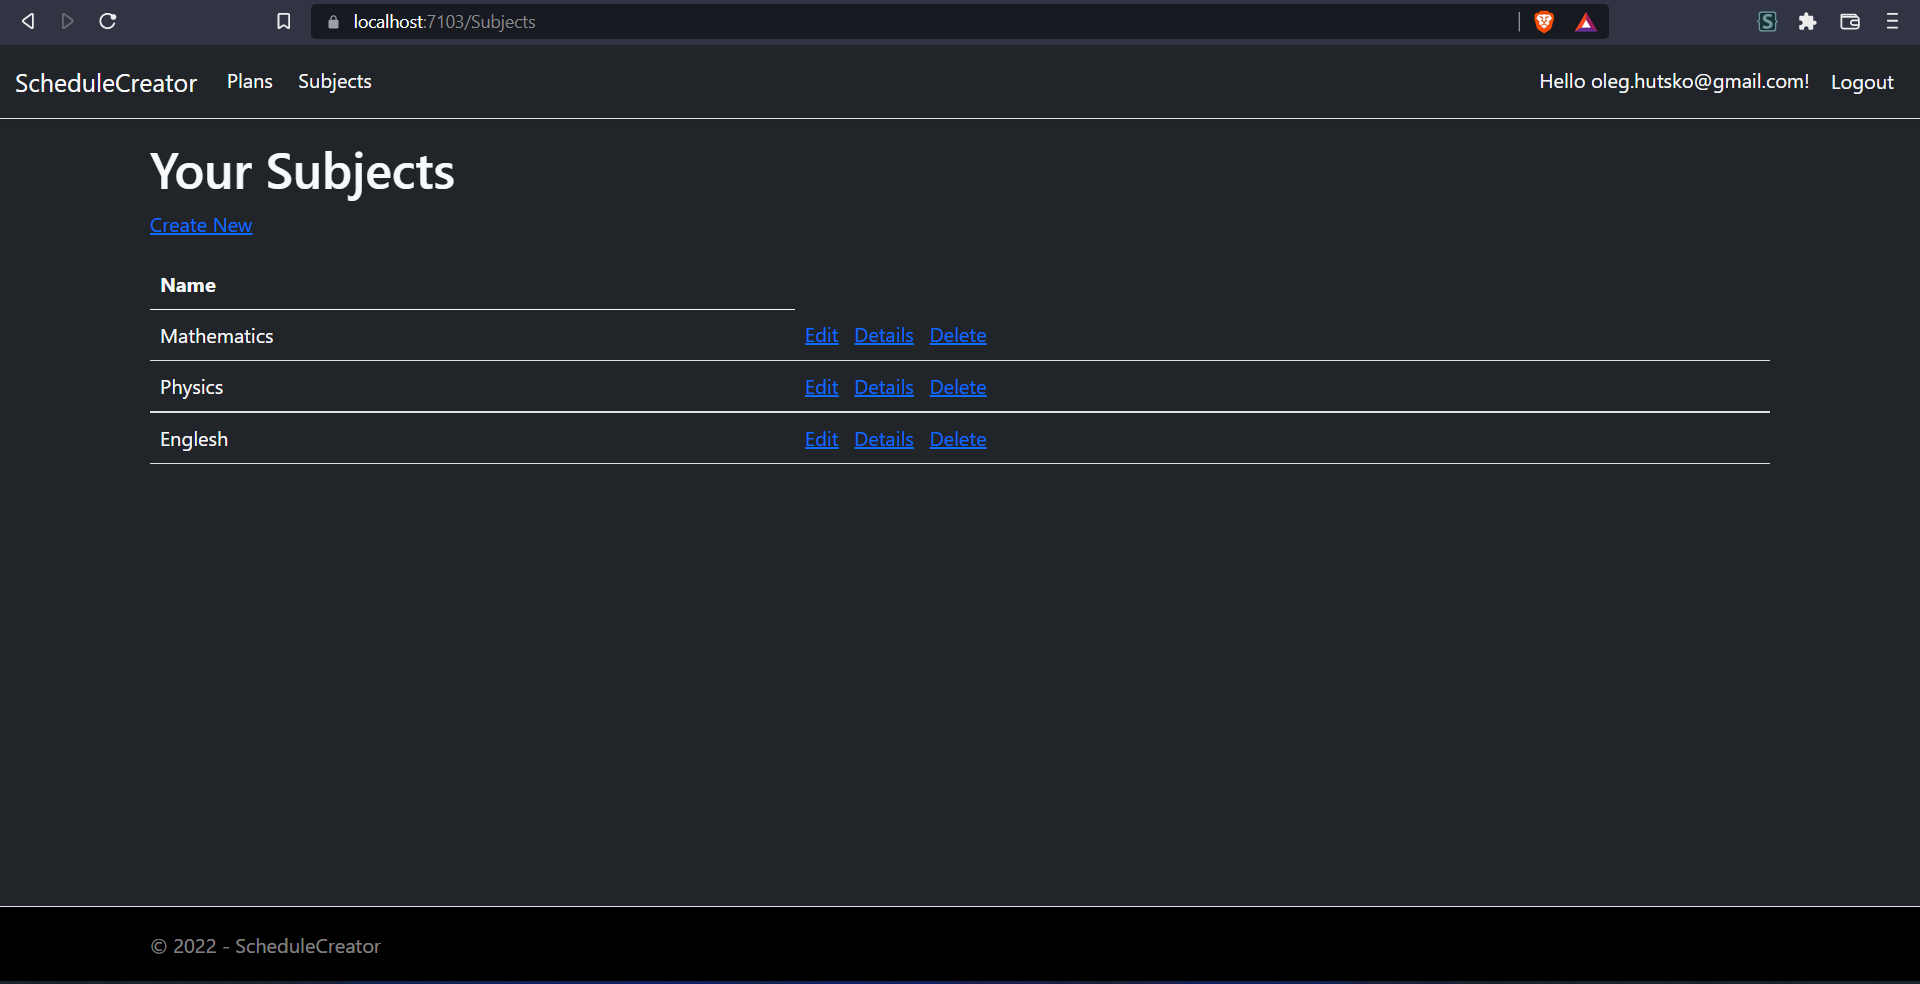
\includegraphics[width=14cm]{8.png}
    \caption{Strona przedmiotów po dodaniu przedmiotów}
\end{figure}

\begin{figure}[h]
    \centering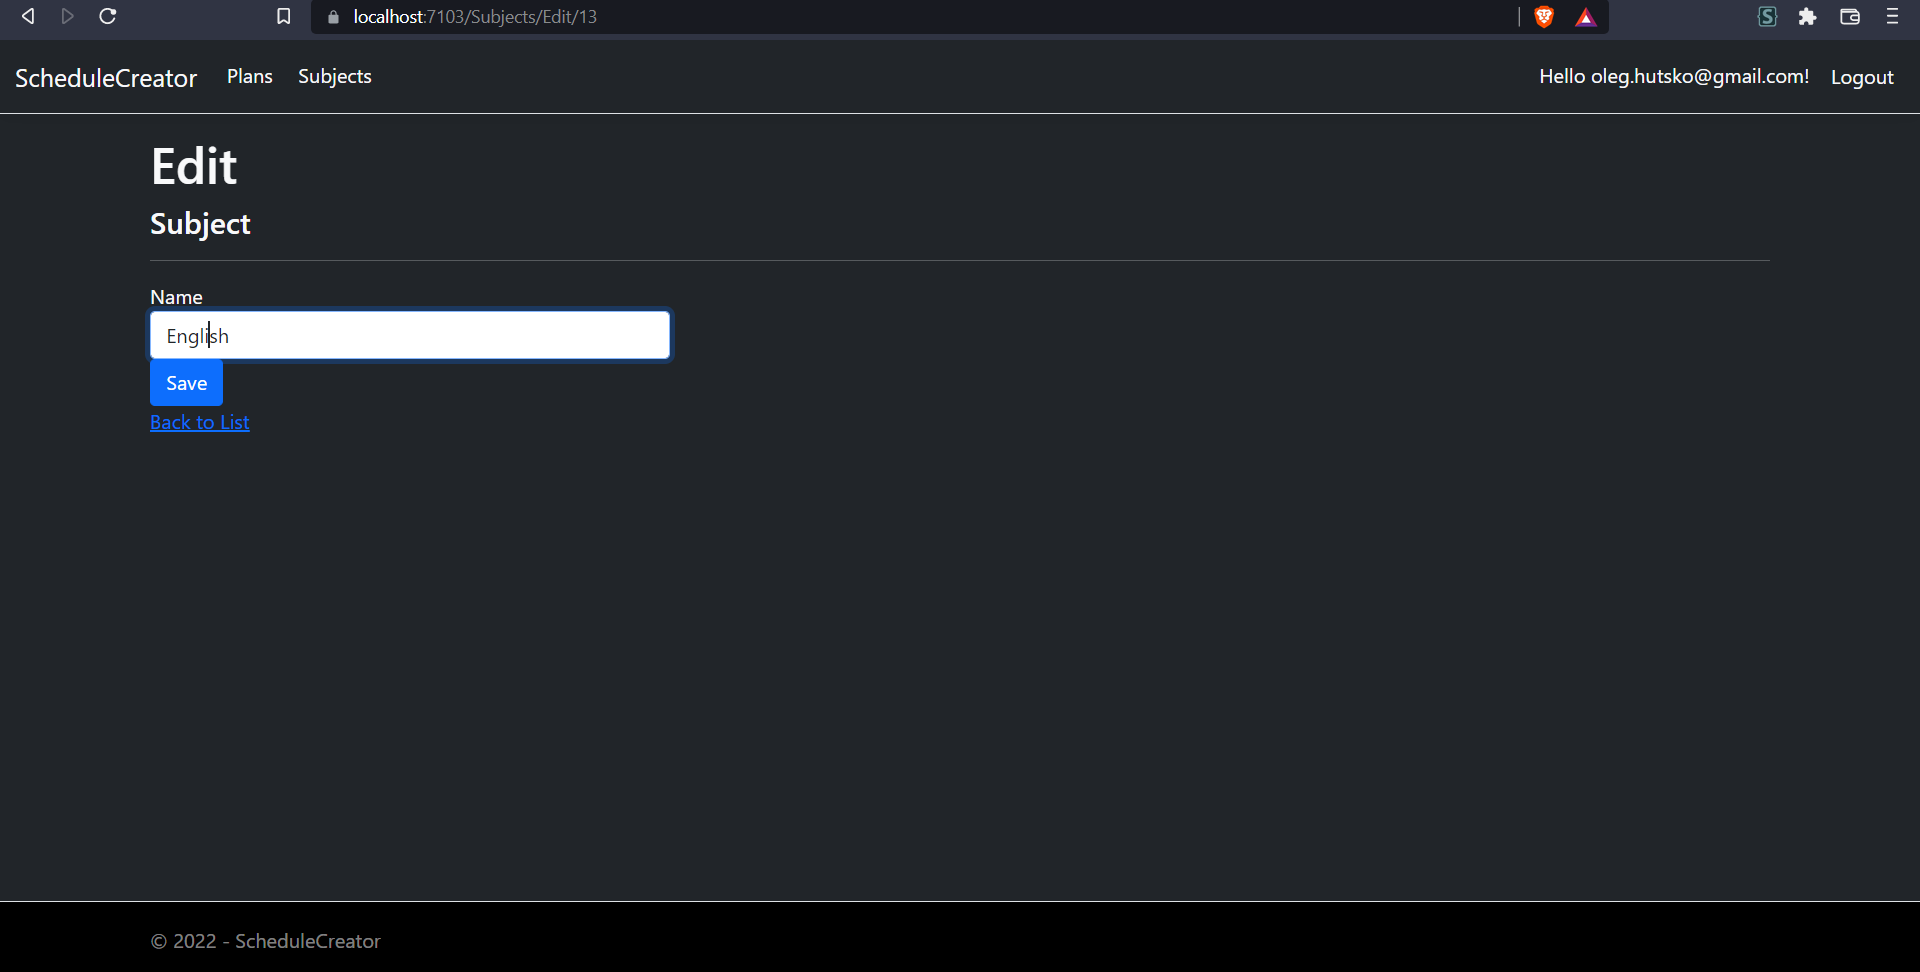
\includegraphics[width=14cm]{9.png}
    \caption{Strona edycji przedmiotów}
\end{figure}

\begin{figure}[h]
    \centering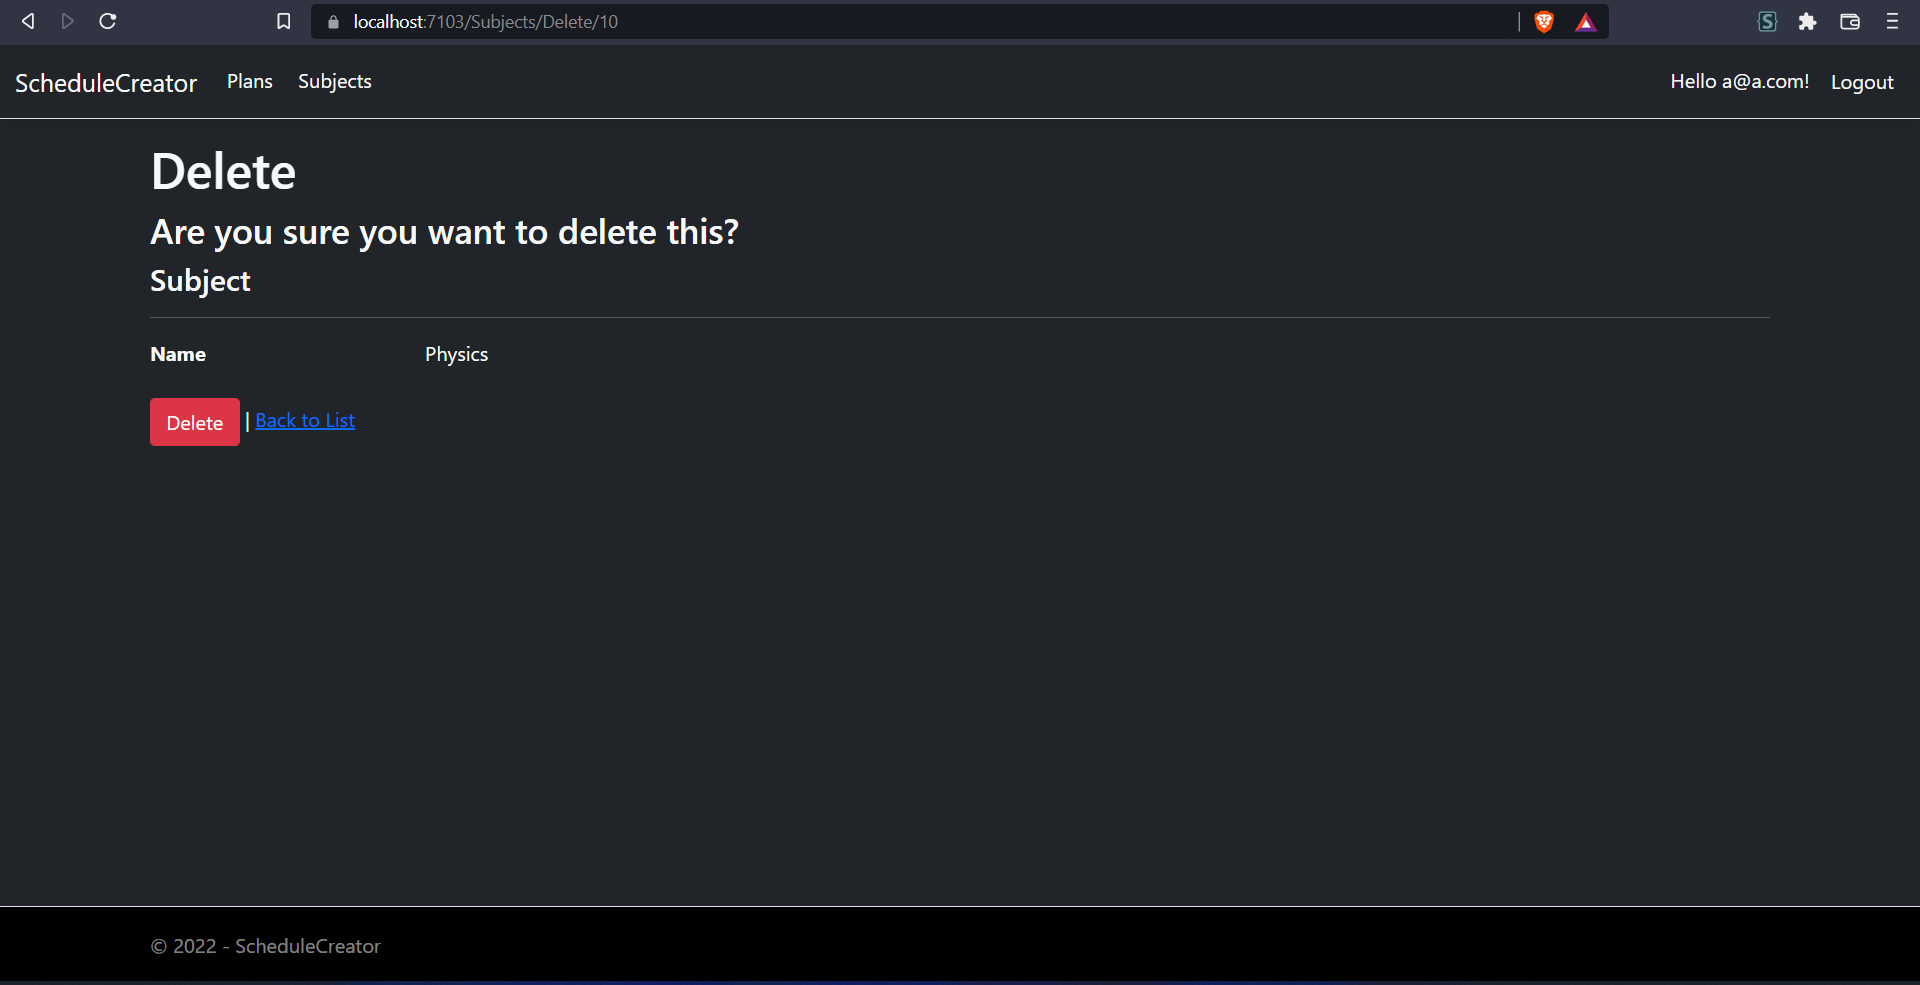
\includegraphics[width=14cm]{10.png}
    \caption{Strona usunięcia przedmiotów}
\end{figure}


\addcontentsline{toc}{chapter}{CRUD przedmioty}
\chapter*{CRUD Planów}

\begin{figure}[h]
    \centering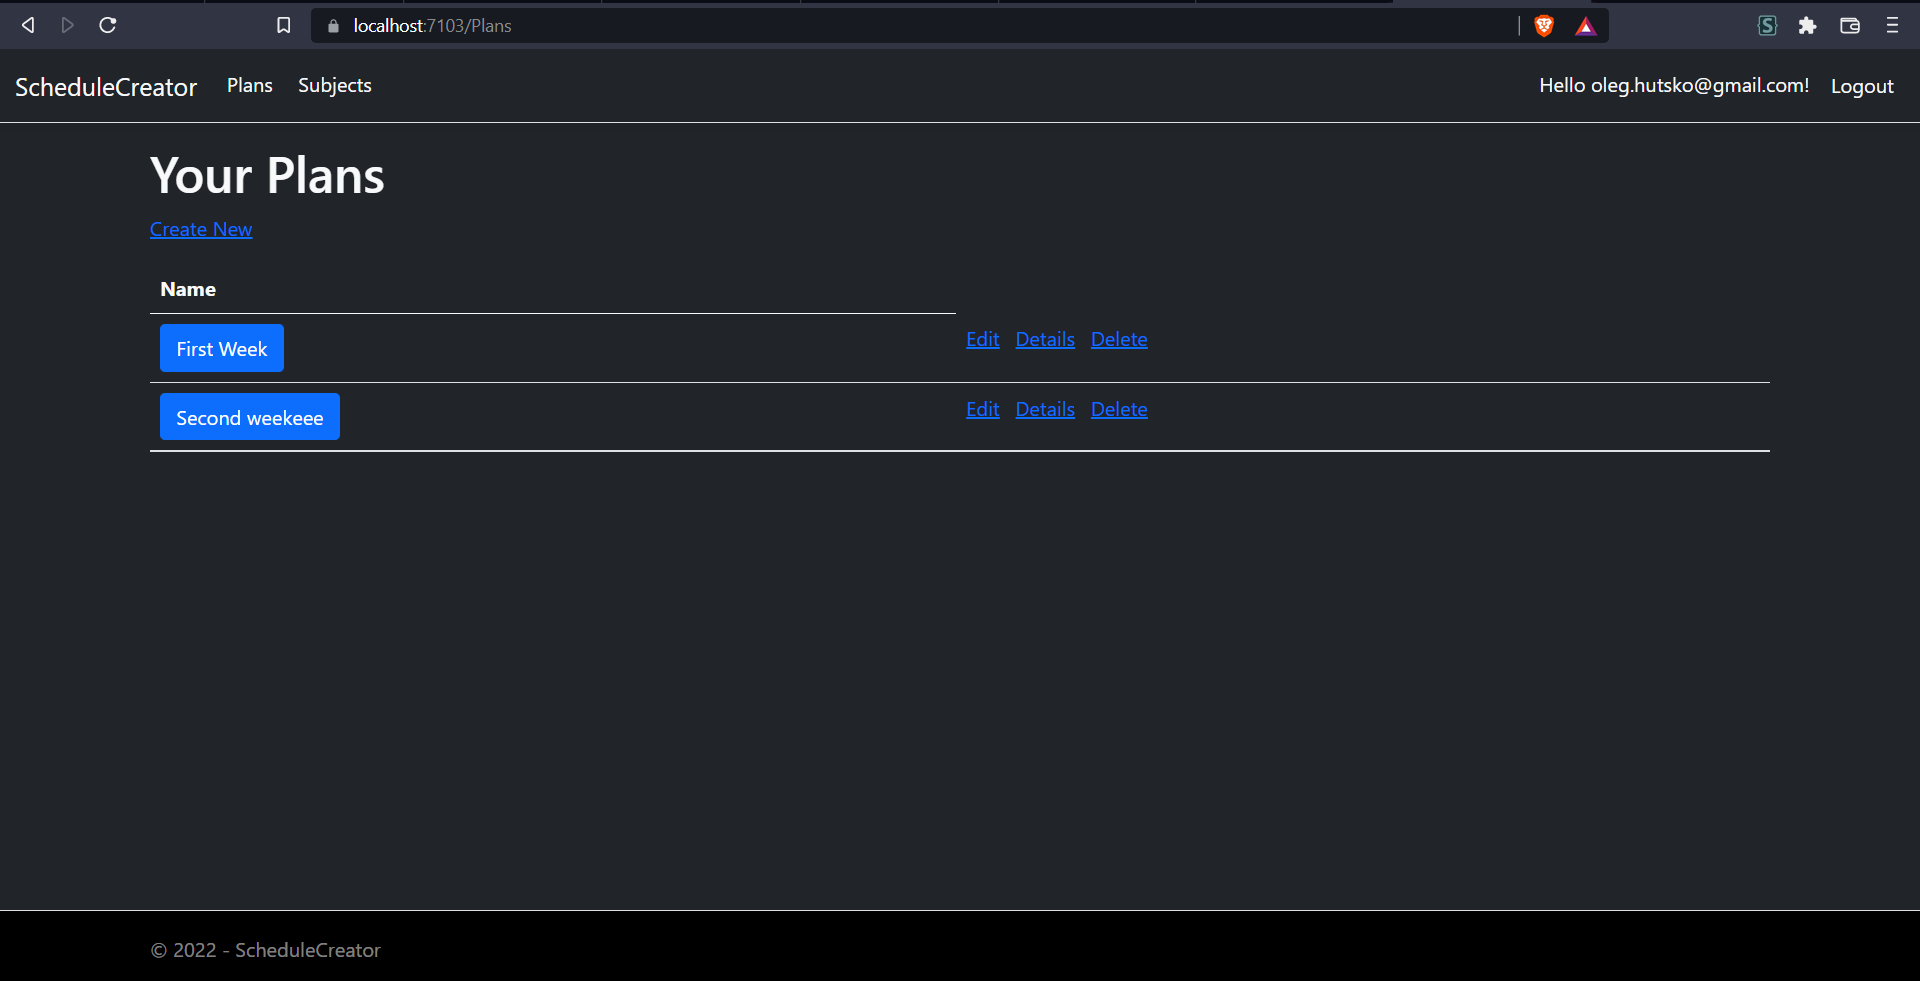
\includegraphics[width=14cm]{16.png}
    \caption{Strona planów }
\end{figure}

\begin{figure}[h]
    \centering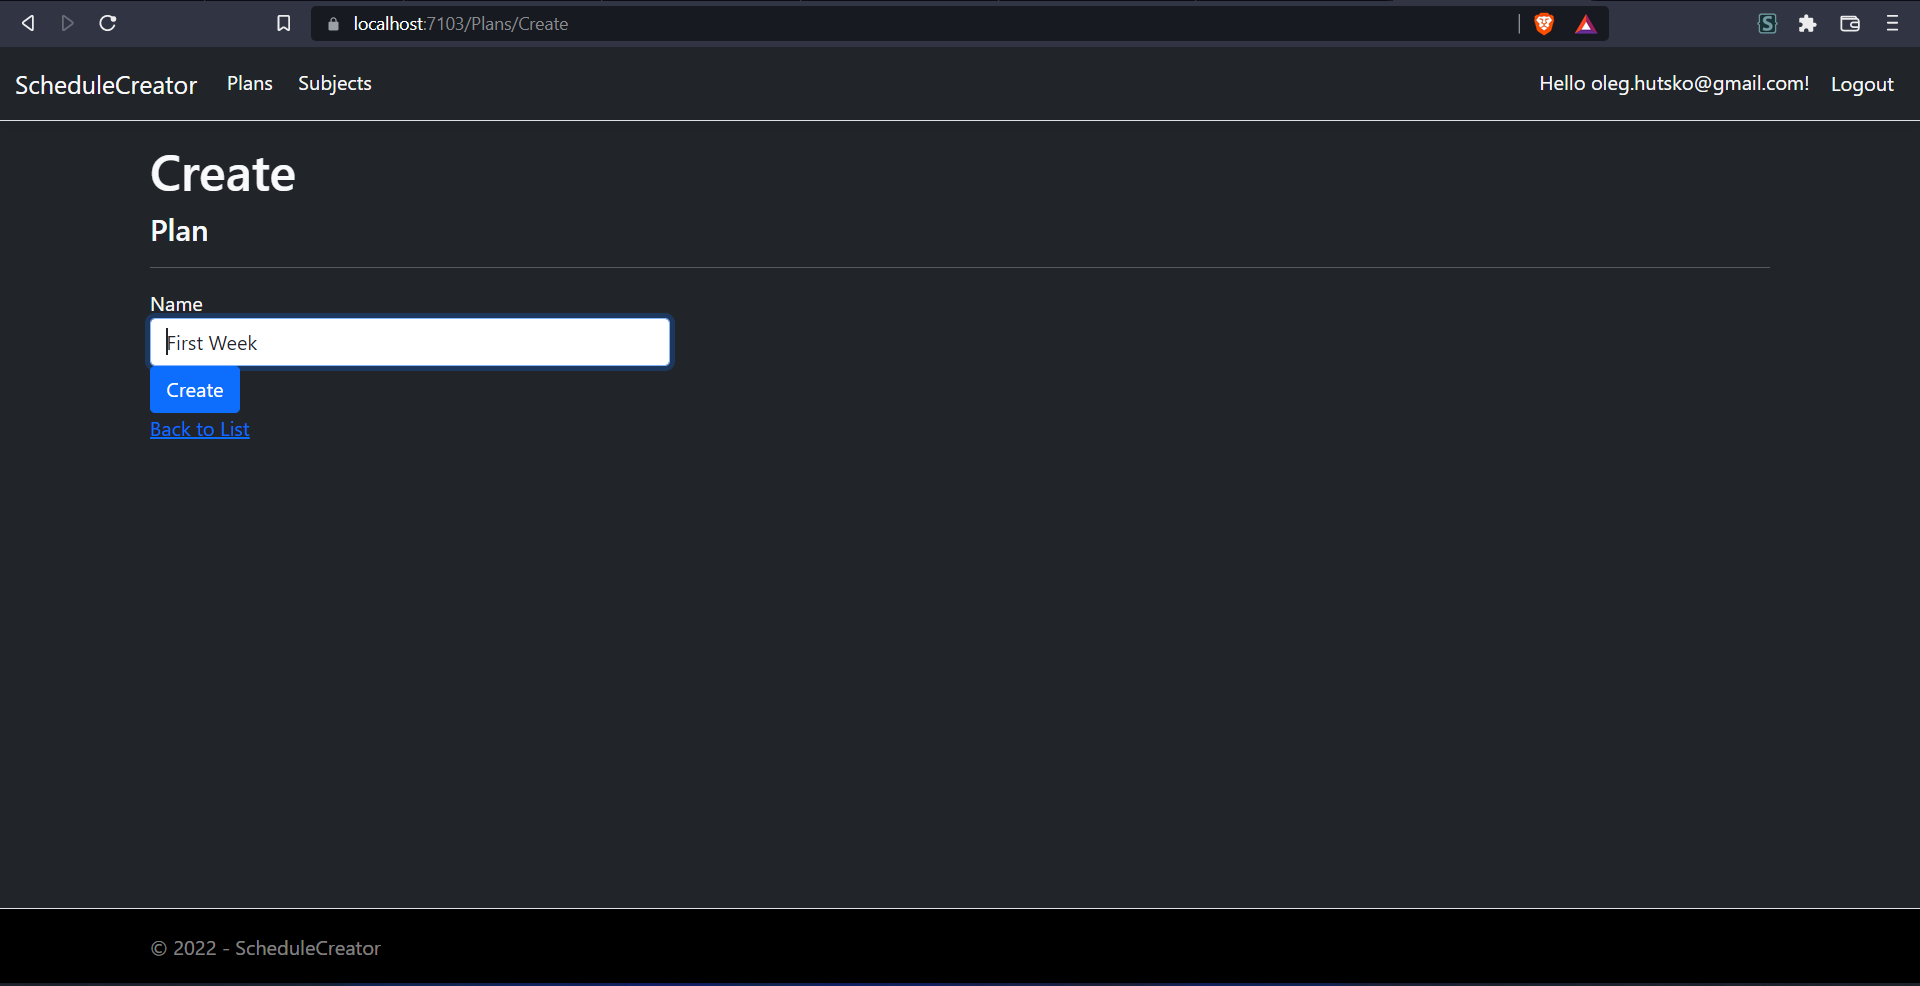
\includegraphics[width=14cm]{12.png}
    \caption{Strona stworzenia nowego planu}
\end{figure}

\begin{figure}[h]
    \centering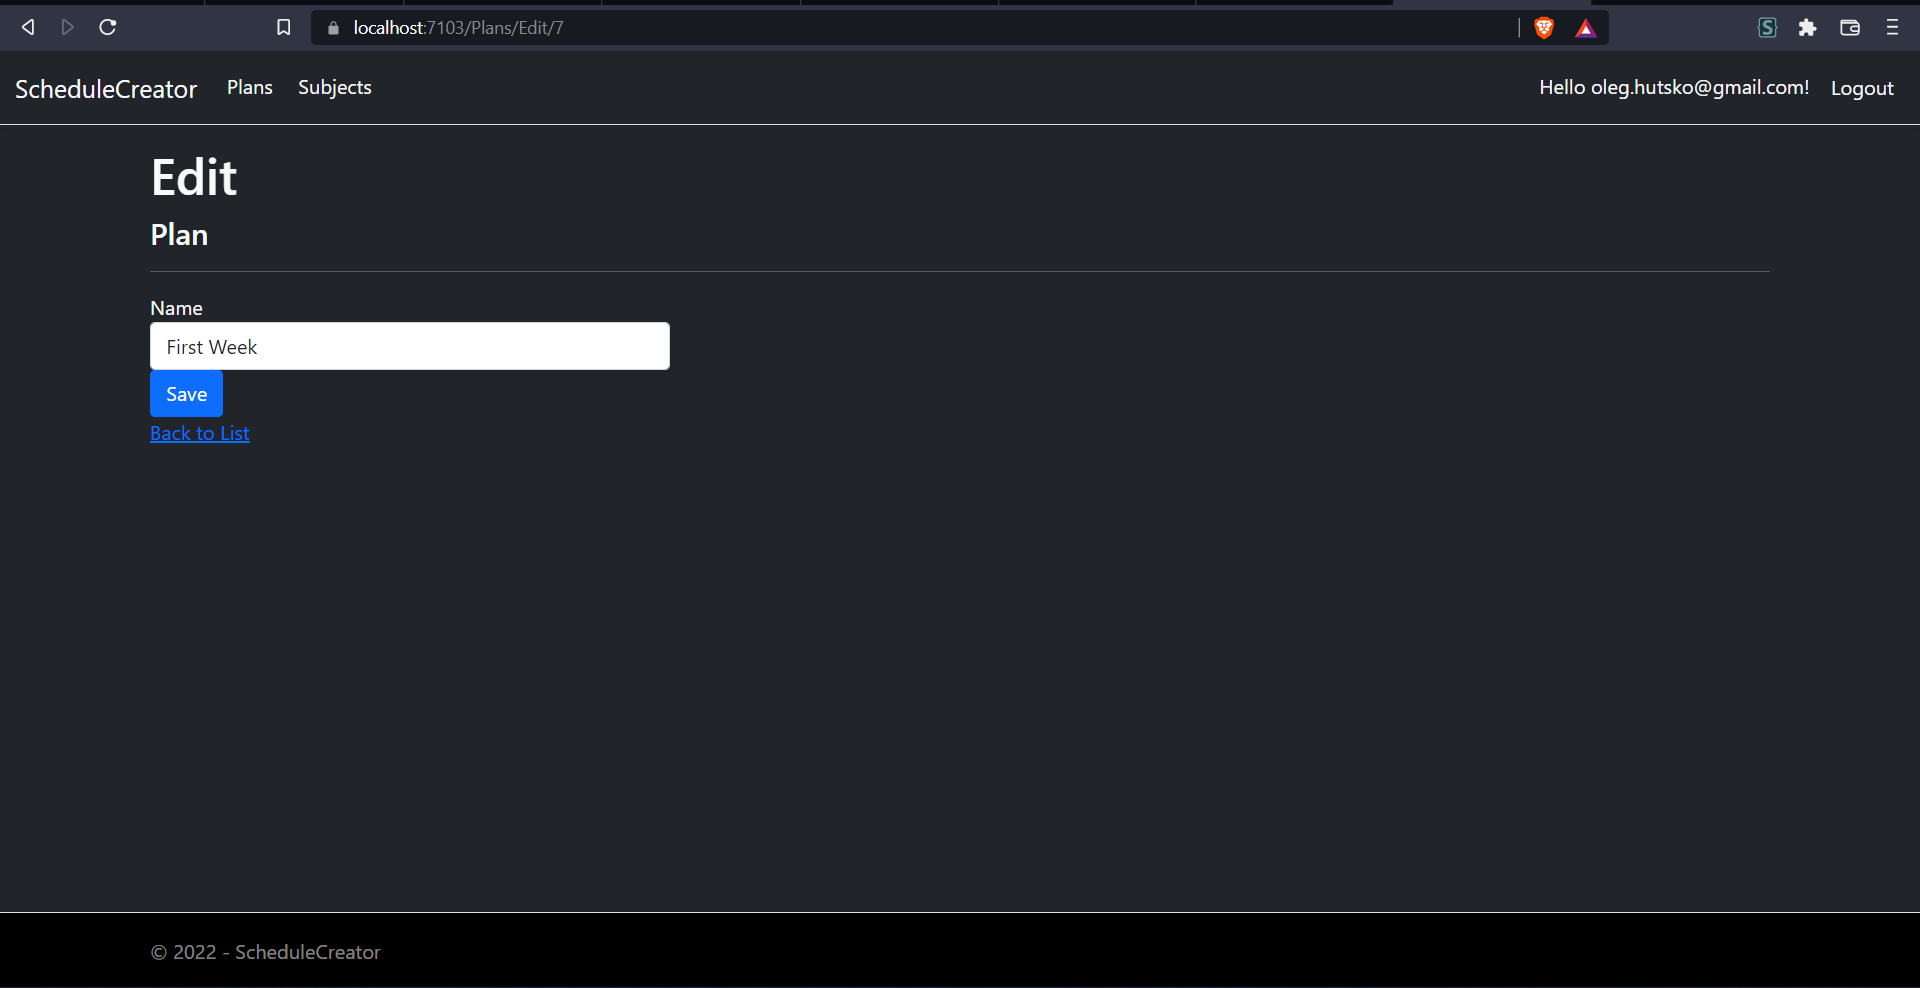
\includegraphics[width=14cm]{13.png}
    \caption{Strona edytowania nowego planu}
\end{figure}

\begin{figure}[h]
    \centering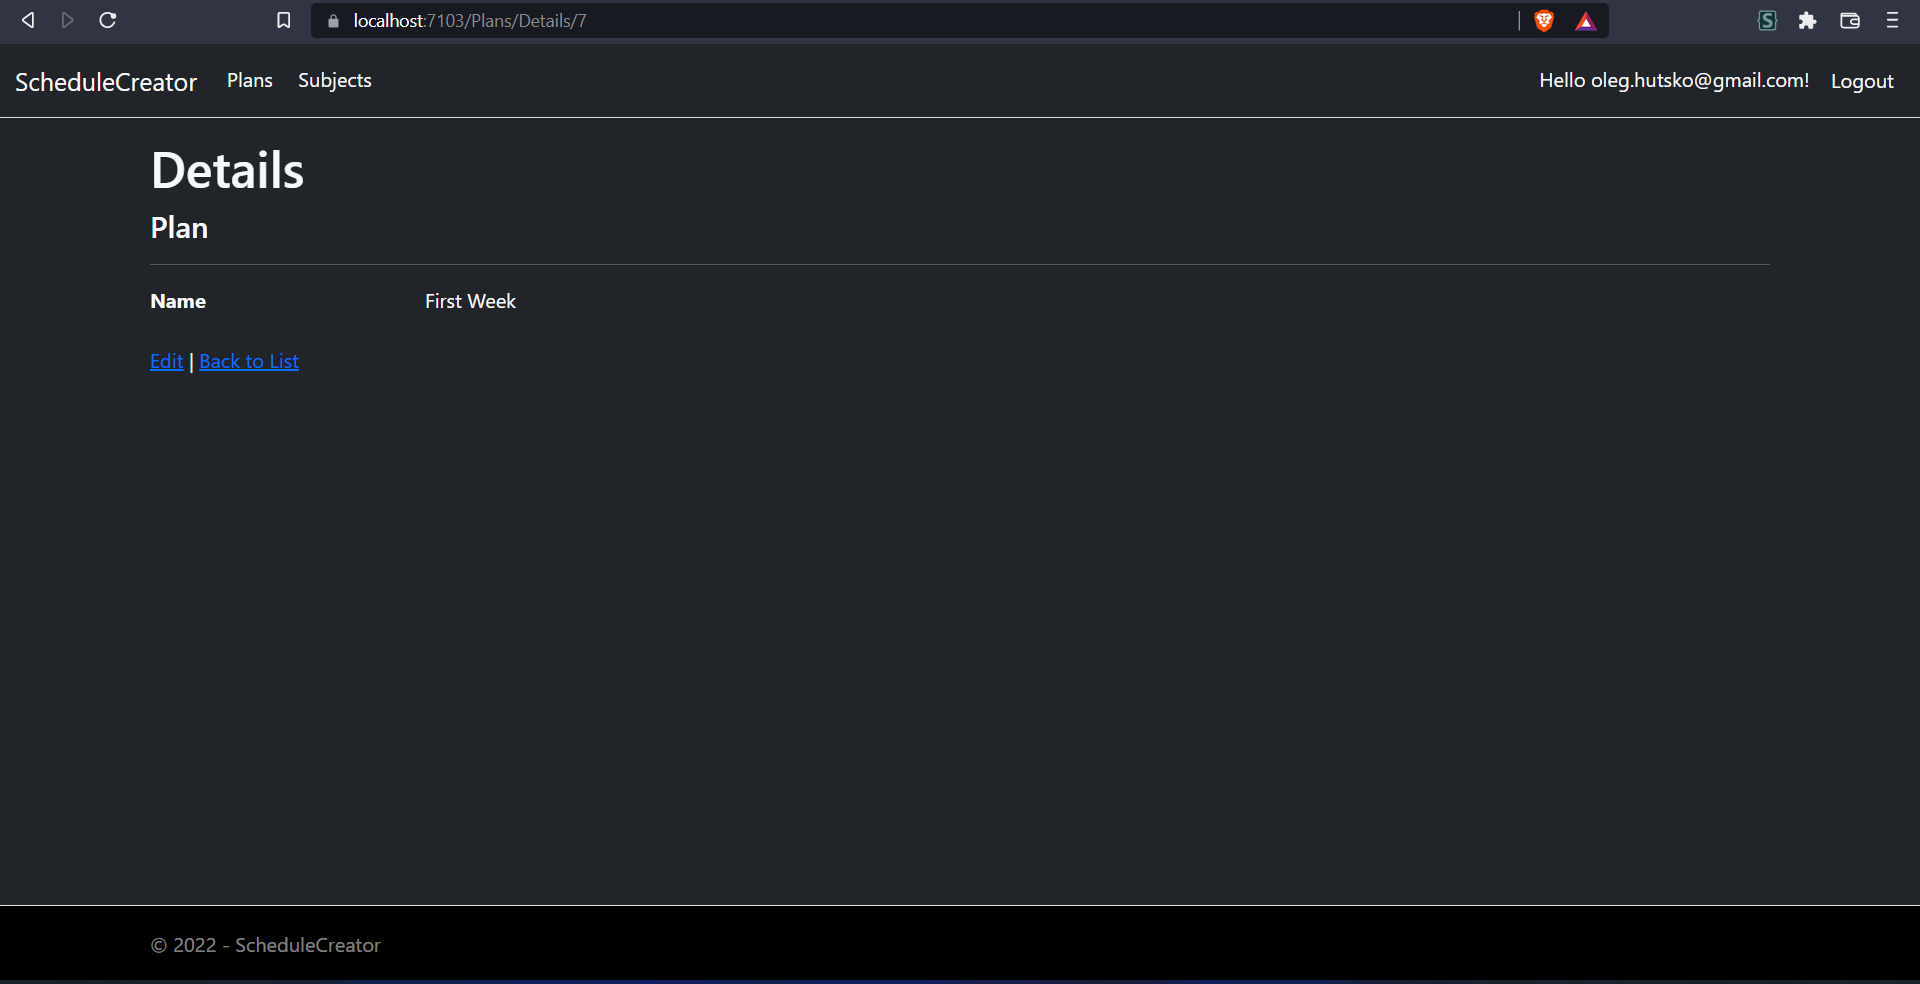
\includegraphics[width=14cm]{14.png}
    \caption{Strona "szczegółów" planu}
\end{figure}

\begin{figure}[h]
    \centering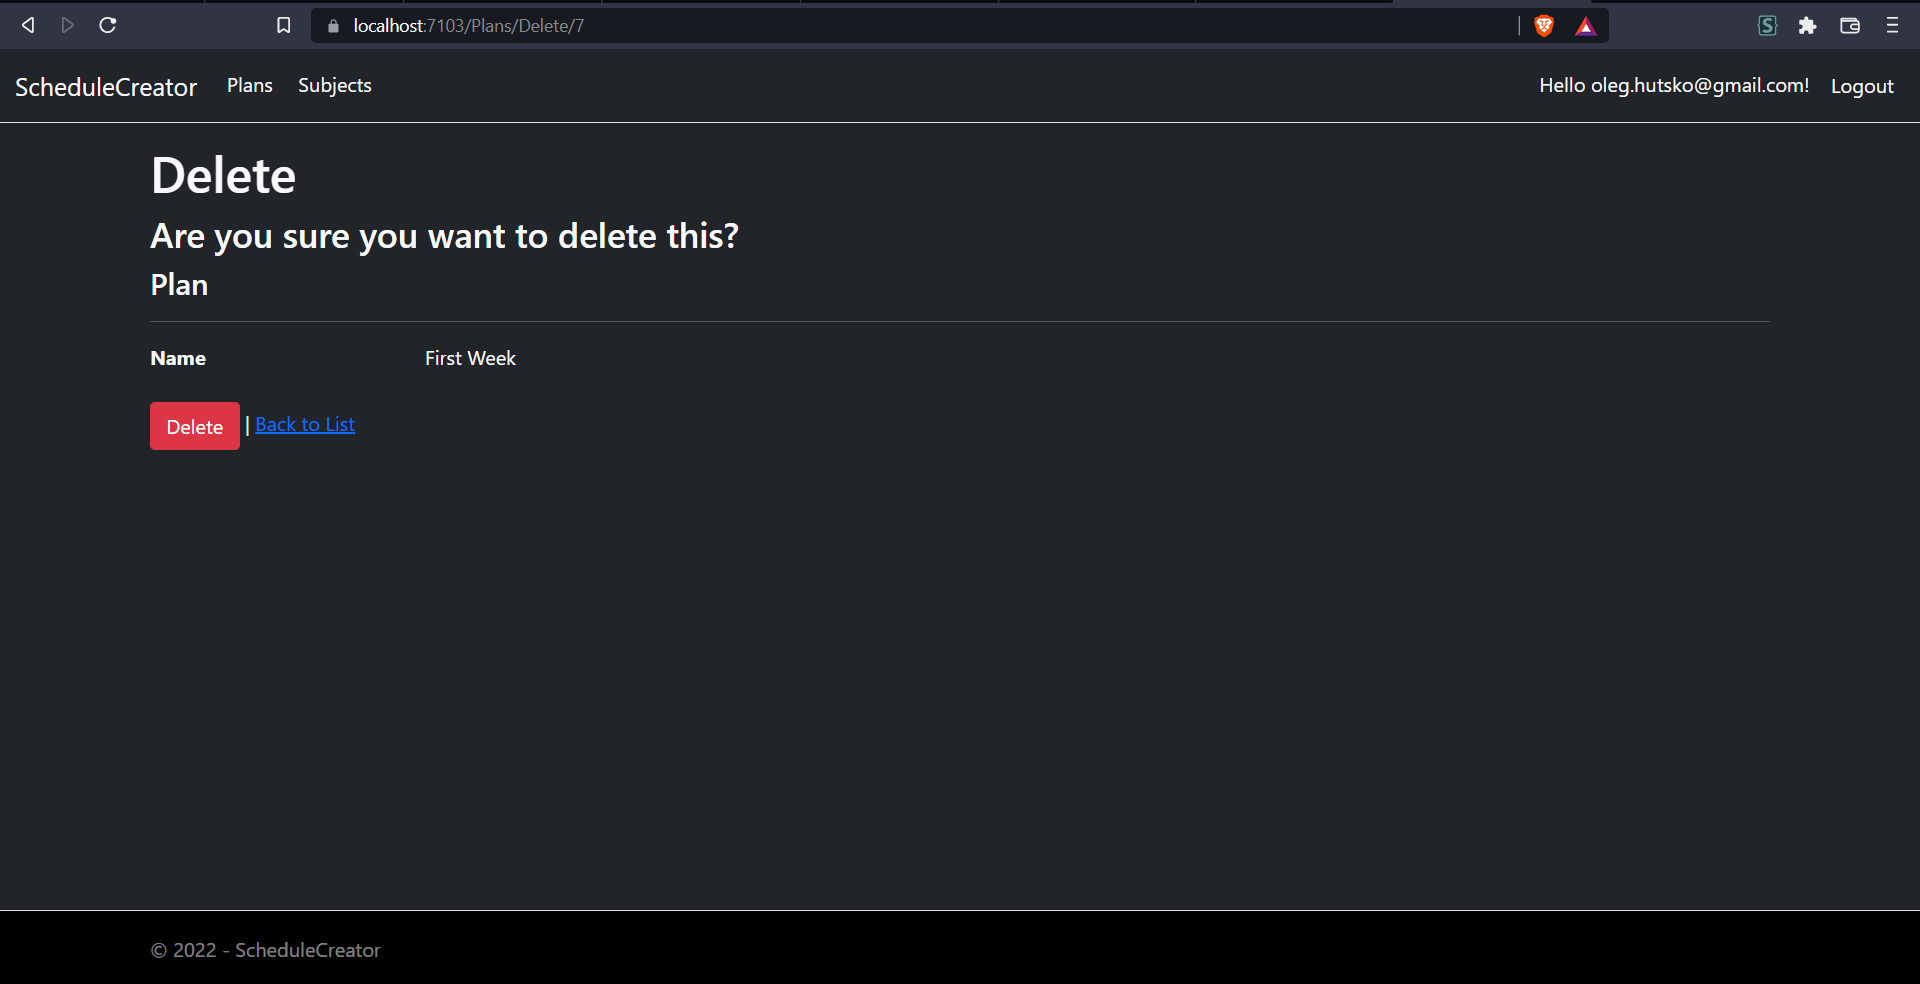
\includegraphics[width=14cm]{15.png}
    \caption{Strona usunięcia planu}
\end{figure}

\addcontentsline{toc}{chapter}{CRUD Planów}
\chapter*{Tworzenie planu}

\begin{figure}[h]
    \centering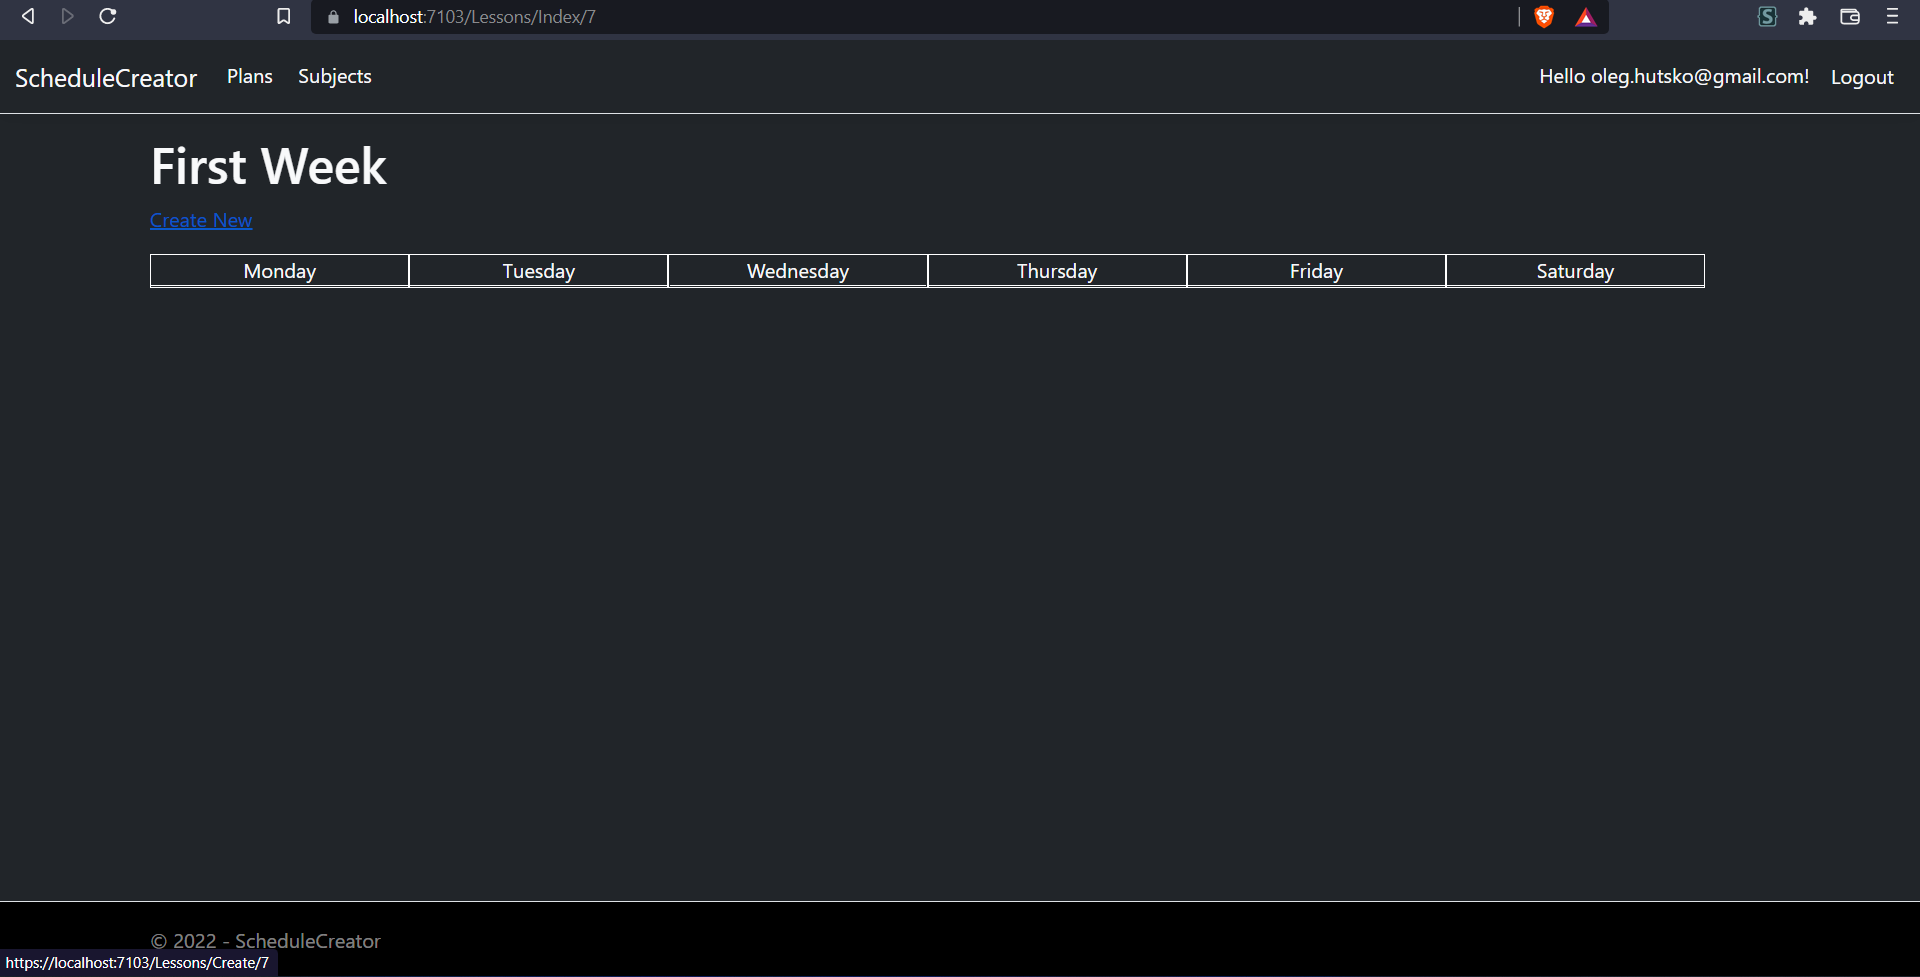
\includegraphics[width=14cm]{17.png}
    \caption{Otwarty pusty plan}
\end{figure}

Zrobiłem stworzenie zajęcia w dwa różne sposoby (w zależnosci od tego, czy użytkownik dodał przedmioty czy nie):
\begin{itemize}
    \item wybór iz komponenty select (dropdownlist) (Rysunek \ref{ref:ddl})
    \item wpisanie ręcznie nazwe przedmiotu (Rysunek \ref{ref:moznapisac})
\end{itemize}
\begin{figure}[h]
    \centering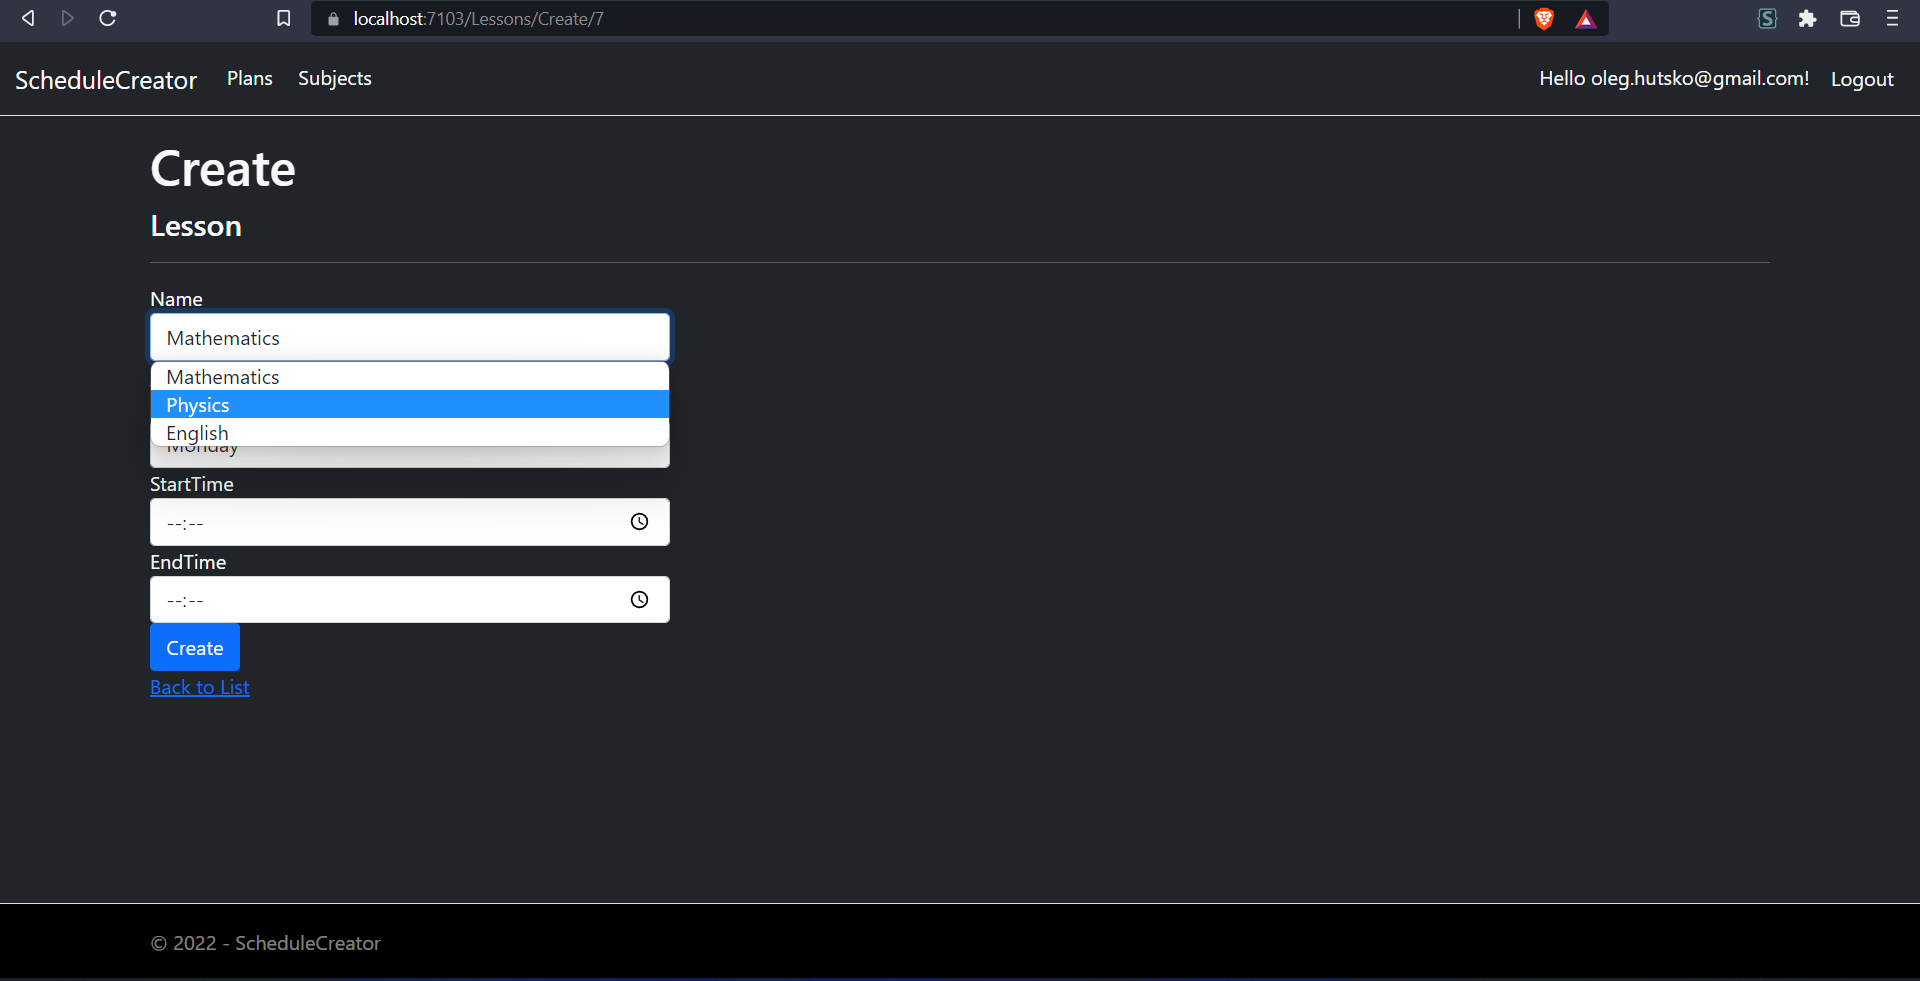
\includegraphics[width=14cm]{18.png}
    \caption{Stworzenie zajęcia na planie}
    \label{ref:ddl}
\end{figure}

\begin{figure}[h]
    \centering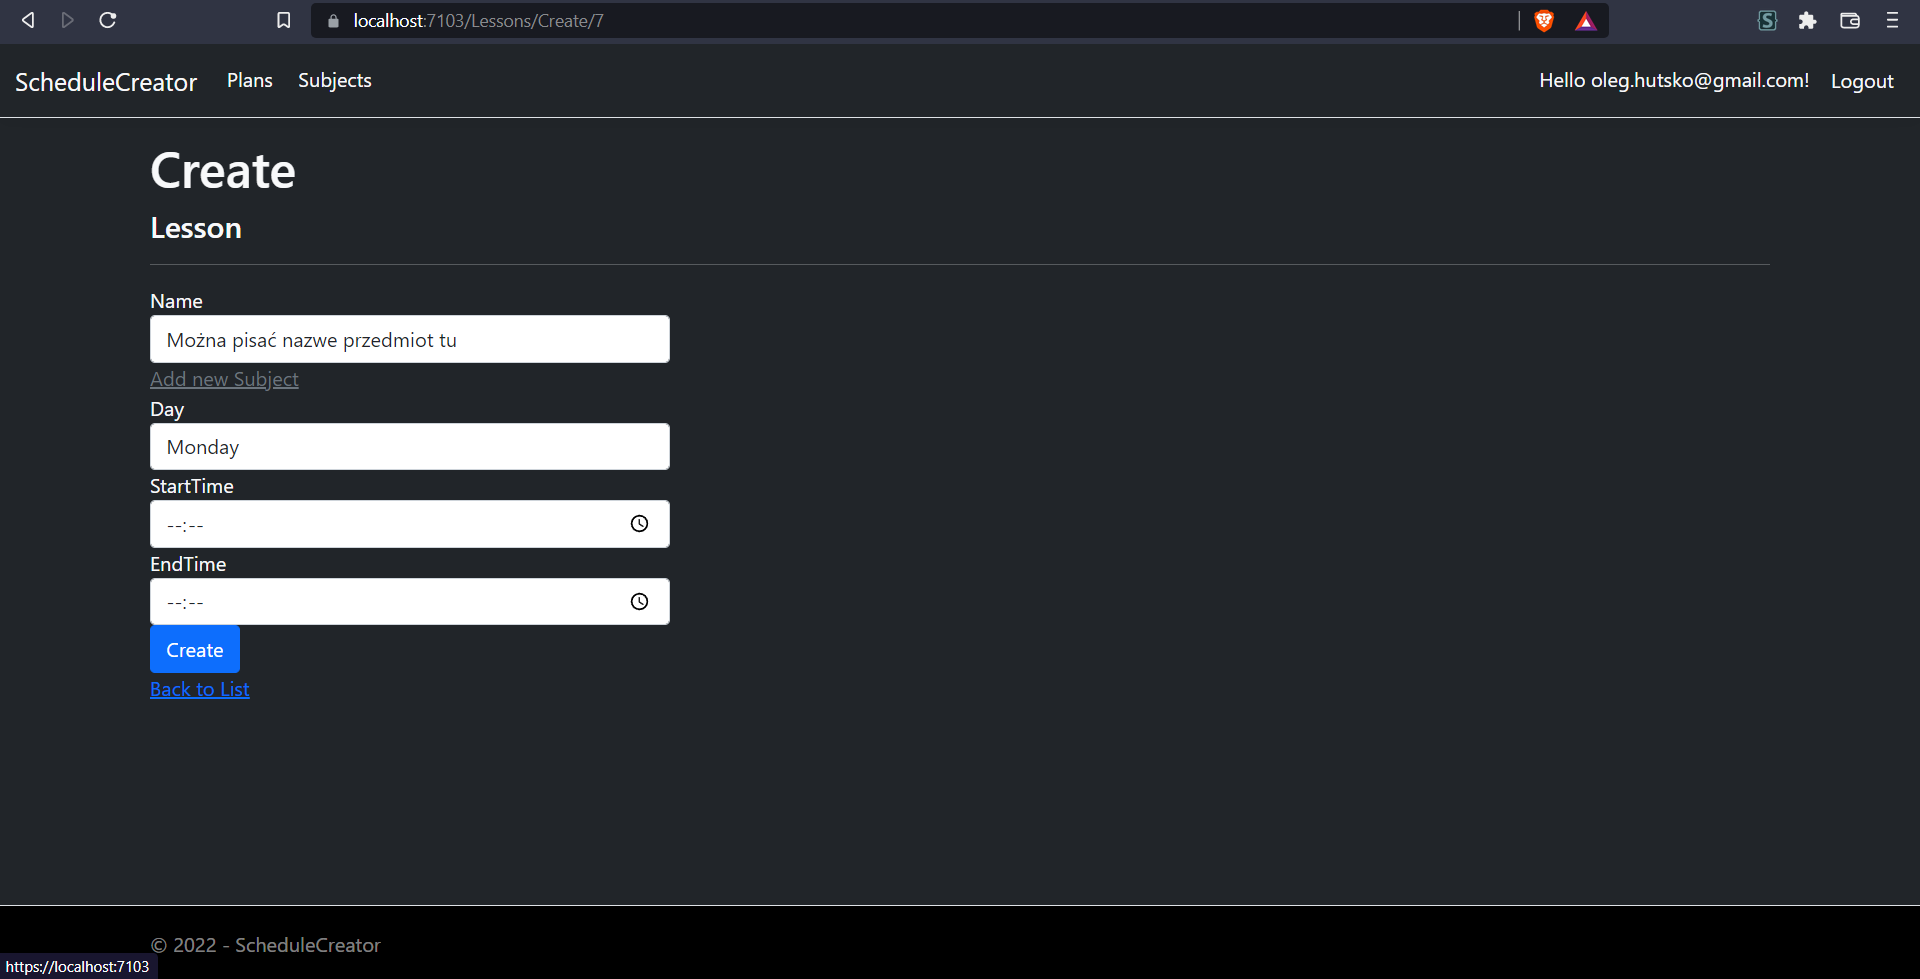
\includegraphics[width=14cm]{moznapisac.png}
    \caption{Stworzenie zajęcia na planie, w przypadku, gdy nie ma przedmiotów}
    \label{ref:moznapisac}
\end{figure}

\begin{figure}[h]
    \centering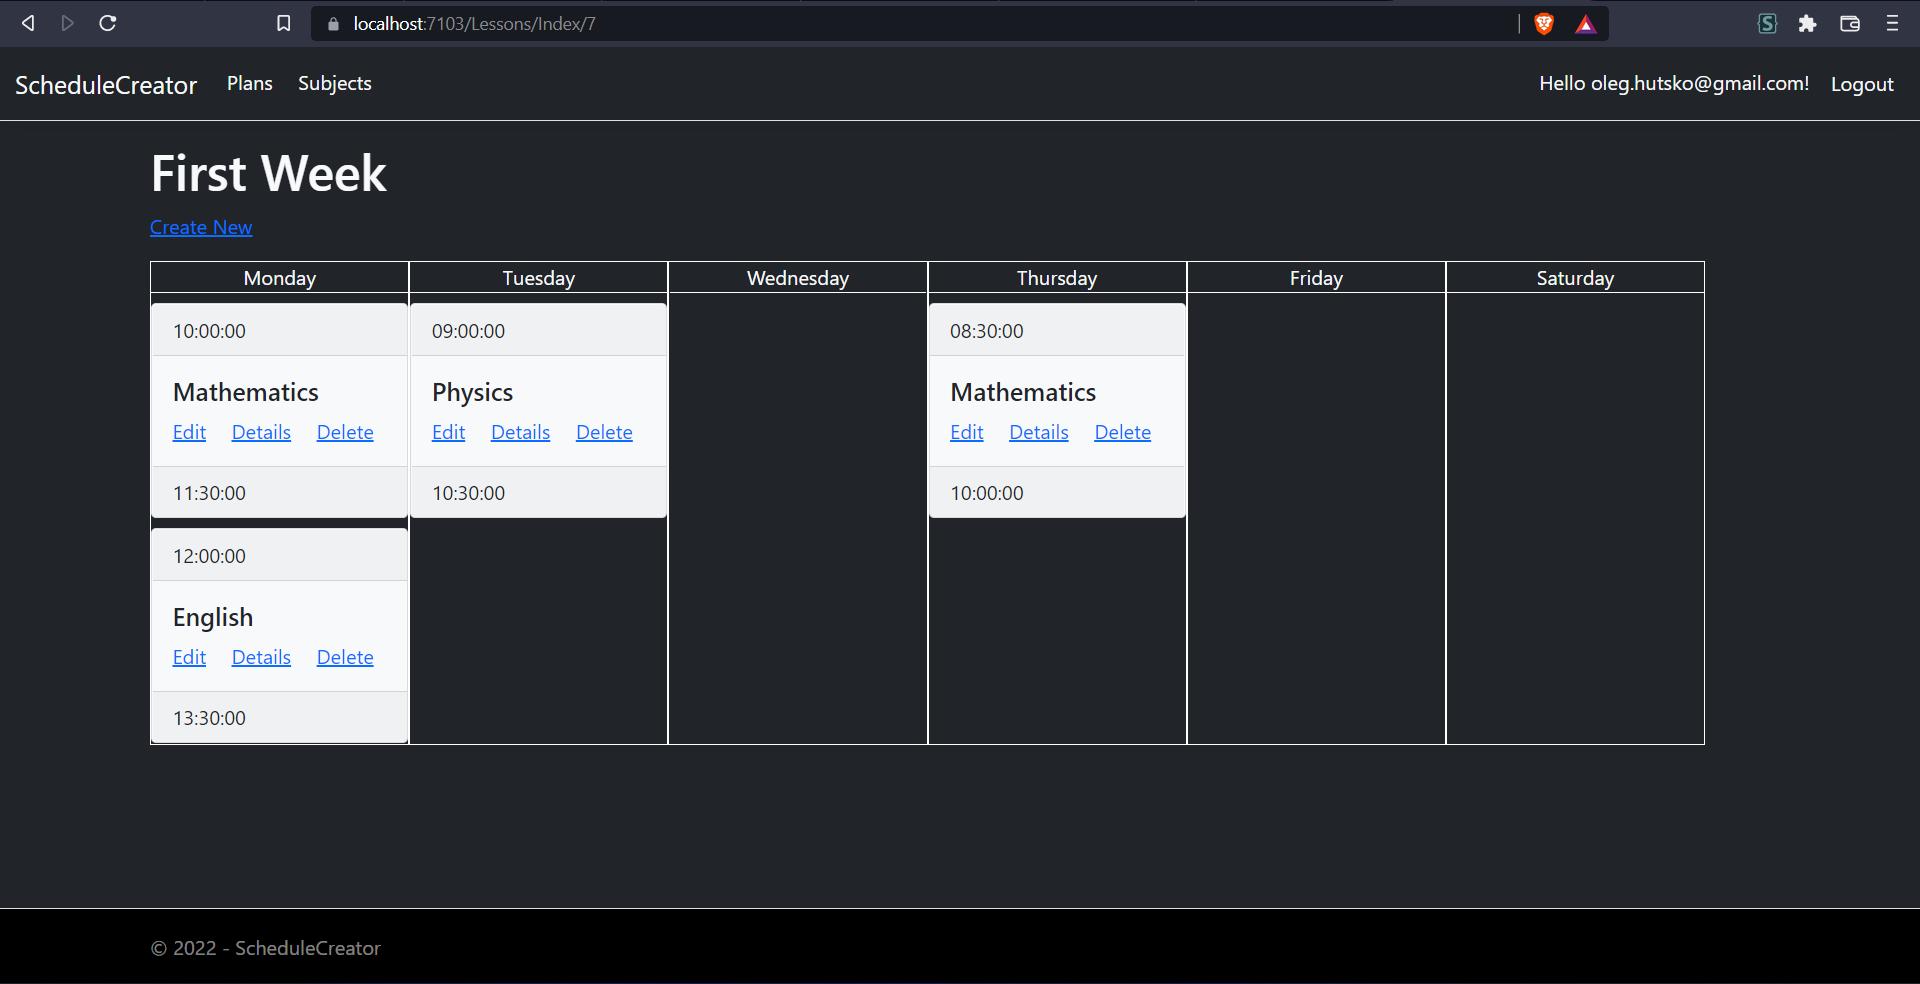
\includegraphics[width=14cm]{20.png}
    \caption{Wypełniony plan zajęć}
\end{figure}

\addcontentsline{toc}{chapter}{Tworzenie planu}
\chapter*{Adaptywność}

Postarałem się zrobić aplikacje tak, żeby wszystkie jej strony było dobrze wyświetlany (za pomocą bootstrap)
\begin{figure}[h]
    \centering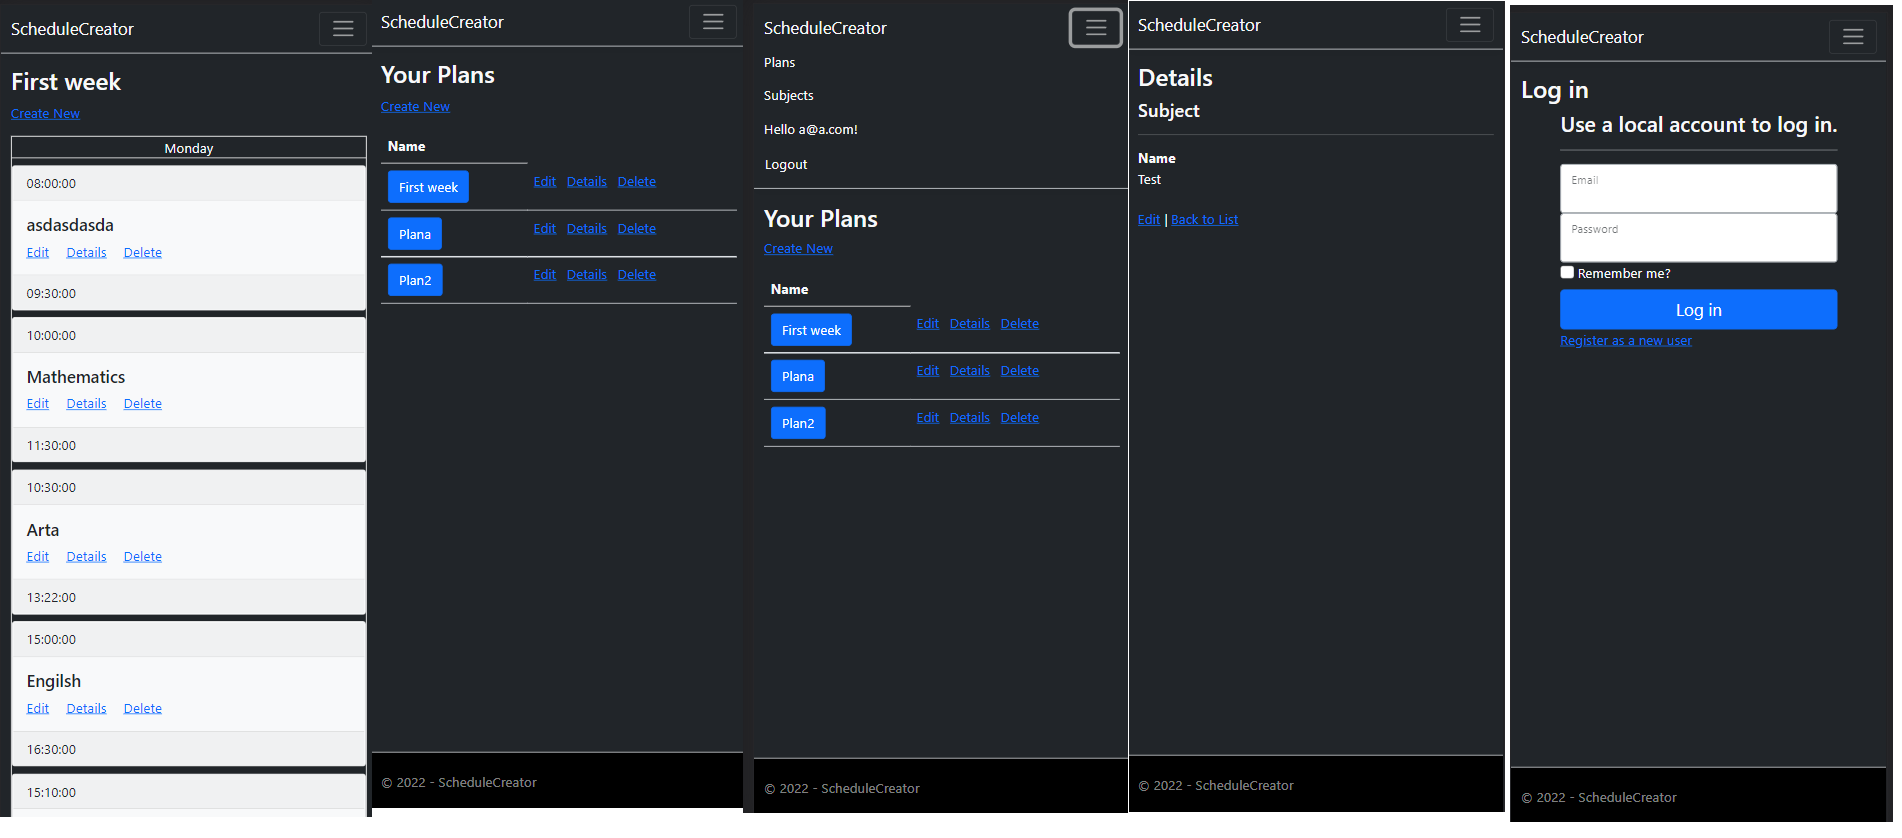
\includegraphics[width=14cm]{mobile.png}
    \caption{Jak aplikacja wygląda na komórce}
\end{figure}

\addcontentsline{toc}{chapter}{Adaptywność}
\chapter*{Wnioski}

Ogólnie rzecz biorąc, budowa strony internetowej z wykorzystaniem MVC sprawiła mi przyjemność, a także pozwoliła nauczyć się nowych umiejętności i rozwinąć stare.
(bootstrap'a, MVC, Entity Framework)

\addcontentsline{toc}{chapter}{Wnioski}
\end{document}